%                                                                 aa.dem
% AA vers. 9.1, LaTeX class for Astronomy & Astrophysics
% demonstration file
%                                                       (c) EDP Sciences
%-----------------------------------------------------------------------
%
%\documentclass[referee]{aa} % for a referee version
%\documentclass[onecolumn]{aa} % for a paper on 1 column  
%\documentclass[longauth]{aa} % for the long lists of affiliations 
%\documentclass[letter]{aa} % for the letters 
%\documentclass[bibyear]{aa} % if the references are not structured 
%                              according to the author-year natbib style

%
\documentclass{aa}  

%
\usepackage{graphicx}
%%%%%%%%%%%%%%%%%%%%%%%%%%%%%%%%%%%%%%%%
\usepackage{txfonts}
%%%%%%%%%%%%%%%%%%%%%%%%%%%%%%%%%%%%%%%%
%\usepackage[options]{hyperref}
% To add links in your PDF file, use the package "hyperref"
% with options according to your LaTeX or PDFLaTeX drivers.
%

\usepackage{color}
\newcommand{\hw}[1]{\textcolor{red}{HW: #1}}
\newcommand{\todo}[1]{\textcolor{green}{TODO: #1}}

\usepackage{amsmath}
\usepackage{subfigure}

\begin{document} 


   \title{Simulating the Universe from the Cosmic Microwave Background to Today}

   \subtitle{}

   \author{A. Martins
          \inst{1}
          }

   \institute{Institute of Theoretical Astrophysics, University of Oslo,
              Sem Sælands vei 13, 0371 Oslo\\
              \email{a.i.s.martins@astro.uio.no}
             }

   \date{}

% \abstract{}{}{}{}{} 
% 5 {} token are mandatory
 
  \abstract
  % context heading (optional)
  % {} leave it empty if necessary  
   {}
  % aims heading (mandatory)
   {We have simulated the large scales of the universe, as well as the recombination and reionisation processes. We then perturbed the initial conditions of the Universe and propagated it through time, in order to simulate the CMB power spectrum.}
  % methods heading (mandatory)
   {We use a Markov chain Monte Carlo to predict the densities of the different components of the Universe, as well as solving ordinary differential equations using a fourth-order Runge-Kutta method. For higher-order ODEs, we use line-of-sight integration.}
  % results heading (mandatory)
   {We find the times of radiation-matter and matter-dark energy equality to be $x=-8.1319$ and $x=-0.25582$. Recombination happens at $x=-7.0$. Perturbations have an oscillatory behaviour that is dampened by the expansion of the Universe. Our simulations of the power spectra agree with observations.}
  % conclusions heading (optional), leave it empty if necessary 
   {}

   \keywords{CMB, Hubble constant, MCMC, Recombination, Reionisation, Linear perturbation theory}

   \maketitle
%
%-------------------------------------------------------------------

\section{Introduction}

\subsection{Background Cosmology}
Since its discovery in 1964 \citep{1965ApJ...142..419P, 1965ApJ...142..414D}, the Cosmic Microwave Background (CMB) is still one of the biggest topics of interest in Cosmology today. The CMB is a black-body radiation spectrum with very small anisotropies that we can observe that was originally released in the early Universe, once photons and matter decoupled and consequently, atoms were formed (and later, once some of these atoms were ionized).

We are interested in simulating the CMB power spectrum in order to fully understand how inflation might have looked like, as well as the recombination and reionization processes. It is useful to start with what the Universe looks like on large scales.

\subsection{Recombination History}

A significant event in the history of the Universe is recombination. In this process, the Universe goes from being made up of a tightly coupled plasma of baryons and photons to having its elements combine into atoms, mostly of Hydrogen and Helium. Photons interacting with atoms is a much less common and significant occurrence than with the previously common electrons and protons, thus making it possible for photons to travel freely and so the CMB is released, letting us observe it today.

\begin{figure*}[ht]
\caption{History of the Universe. Credit: NAOJ}             
\label{fig:history}      
\centering          
\includegraphics[width=\textwidth]{report/figures/eso1620a.jpg}
\end{figure*}

\subsection{Perturbations}

However, life is never that simple, and the Universe is not simply smooth. As such, we need to introduce perturbation theory by adding small perturbations to the initial conditions of our parameters and observing how they evolve until today.

\subsection{Power Spectrum}

With all the elements set up, all that is left to do is build power spectra for the CMB (temperature and polarization) and for matter. This is useful because these are observable quantities from CMB and galaxy survey experiments, meaning we will be able to compare our simulations to real data and verify if they agree.

\section{Theoretical Background}

\subsection{Background Cosmology}

We start by assuming that, at large scales, matter is homogeneous and isotropic. The mathematical formulation of this, i.e. the metric that describes the geometry of the Universe at large scales is given by the Friedmann–Lemaître–Robertson–Walker (FRLW) metric:
\begin{equation}
ds^2 = -dt^2 + a^2(t)(dx^2 + dy^2 + dz^2),
\end{equation}
where $a(t)$ is the scale factor of the Universe, a measure for the rate of its expansion.

We are interested in learning about the densities of the different components of the Universe at different points in time, from the Cosmic Microwave Background until the present day. The $\Lambda$CDM model assumes that the Universe is composed of matter (baryons\footnote{Baryons in this context refers to all "normal" matter, i.e. quarks, leptons (not including neutrinos for our purposes) and combinations of them.} and cold, dark matter (CDM)), radiation (photons and massless neutrinos) and dark energy. Another important notion for our model is that of curvature, which we already implicitly assumed to be 0 in the above equation, i.e. we are assuming a flat Universe. These components come together in the Friedman equation, which relates their density evolution to the expansion of the Universe:
\begin{equation}
H(a) = H_0 \sqrt{\Omega_{M0}a^{-3} + \Omega_{R0}a^{-4} + \Omega_{k 0} a^{-2} + \Omega_{\Lambda 0}},
\end{equation}
where $H(a)$ is the so-called Hubble parameter and $H_0$ is the Hubble constant, whose value is contested and has been measured experimentally to be anywhere from 67 to 74 km/s/Mpc (\cite{hu2023hubbletensionevidencenew}). Each $\Omega_{i0}$ represents the density of one of the above-mentioned components in the present day, now explicitly including curvature $k$, and $\Omega_{M0} = \Omega_{b0} + \Omega_\text{CDM0}, \Omega_{R0} = \Omega_{\gamma0} + \Omega_{\nu0}$. The densities for photons and neutrinos today are given by
\begin{align}
\Omega_{\gamma 0} &= 2\cdot \frac{\pi^2}{30} \frac{(k_bT_{\rm CMB 0})^4}{\hbar^3 c^5} \cdot \frac{8\pi G}{3H_0^2},\\
\Omega_{\nu 0} &= N_{\rm eff}\cdot \frac{7}{8}\cdot \left(\frac{4}{11}\right)^{4/3}\Omega_{\gamma 0},
\end{align}
whereas the densities for baryons and CDM are assumed to be, respectively, 0.05 and 0.267, the values given by \cite{2020}. The densities of all the components need to, of course, add up to one. We then find that 
$\Omega_{\Lambda 0} = 1 - (\Omega_{b 0}+\Omega_{\rm CDM 0}) - (\Omega_{\gamma 0} + \Omega_{\nu 0}) - \Omega_{k 0}$, where, assuming a flat universe, $\Omega_{k 0} = 0$.

We can get the component densities for different scale factors from
\begin{equation}
\label{eq:omegas}
\begin{aligned}
\Omega_{k}(a) &= \frac{\Omega_{k0}}{a^2H(a)^2/H_0^2}\\
\Omega_{\rm CDM}(a) &= \frac{\Omega_{\rm CDM 0}}{a^3H(a)^2/H_0^2} \\
\Omega_b(a) &= \frac{\Omega_{b 0}}{a^3H(a)^2/H_0^2} \\
\Omega_\gamma(a) &= \frac{\Omega_{\gamma 0}}{a^4H(a)^2/H_0^2} \\
\Omega_{\nu}(a) &= \frac{\Omega_{\nu 0}}{a^4H(a)^2/H_0^2} \\
\Omega_{\Lambda}(a) &= \frac{\Omega_{\Lambda 0}}{H(a)^2/H_0^2}.
\end{aligned}
\end{equation}

It is handy to explore the Hubble parameter equations before introducing some new notions. In particular, a useful quantity is the scaled Hubble parameter $\mathcal H = aH$. Differentiating this with respect to $x = \log a$ and denoting the derivative with respect to $x$ as ', we have
\begin{align}
    \mathcal H' &= \frac{d\mathcal H}{dx} = \frac{da}{dx}\frac{d\mathcal H}{da}\\ 
    &= a\left( H(a) + \frac{1}{2}\frac{aH_0^2}{ H(a)} (-3\Omega_{M0} a^{-4} - 4\Omega_{R0}a^{-5}-2\Omega_{k0}a^{-3})\right)\\
    &= \mathcal H(x) +\frac{1}{2}\frac{(e^xH_0)^2}{\mathcal H(x)}(-3\Omega_{M0} e^{-3x} - 4 \Omega_{R0}e^{-4x}-2\Omega_{k0}e^{-2x}).
\end{align}

Differentiating once more, we get
\begin{alignat*}{2}
    \mathcal H'' &= \frac{d^2\mathcal H}{dx^2}&&\\ 
    %&= \mathcal H'\Bigg(1-&&\frac{1}{4}\left(\frac{e^xH_0}{\mathcal H(x)}\right)^5\\
    %& &&(3\Omega_{M0}e^{-3x}+4\Omega_{R0}e^{-4x}+2\Omega_{k0}e^{-2x})^2\\
    %& &&(9\Omega_{M0}e^{-3x}+16\Omega_{R0}e^{-4x}+4\Omega_{k0}e^{-2x})\Bigg).
    &= \frac{H_0^2}{2\mathcal{H}}\left(-\Omega_{M0} e^{-x}-2\Omega_{R0}e^{-2x}+2\Omega_{\Lambda0}e^{2x}\right) \\&-\frac{H_0^4}{4\mathcal{H}^3}\left(\Omega_{M0}e^{-x}+4\Omega_{R0}e^{-2x}+4\Omega_{\Lambda0}e^{2x}\right)^2.
\end{alignat*}

It is now useful to define the notion of conformal time $\eta$, the distance the light has traveled since the Big Bang until a certain time $x$, taking into account the expansion of the Universe. A differential equation for $\eta$ can be written as
\begin{align}
\frac{d\eta}{dx} = \frac{da}{dx}\frac{d\eta}{da} = \frac{c}{\mathcal{H}}.
\end{align}

From this, follow the definition of the co-moving distance $\chi$, the distance between the observer and a measurable quantity:
\begin{align}
\chi = \eta_0 - \eta
\end{align}

We can define the luminosity distance, i.e. given the intrinsic luminosity of a source and its flux, the distance to the source is
\begin{equation}
d_L = \frac{d_A}{a^2},
\end{equation}
where $d_A = \frac{\chi}{1+z}$ is the angular diameter distance that defines the angular size of an object at redshift $z$.

For a flat Universe, this reduces to
\begin{equation}
    d_L = \frac{\chi}{a}.
\end{equation}

A last useful notion before we get into some deductions is that of cosmic time $t$, which is given by solving
\begin{align}
\label{eq:t-ode}
\frac{dt}{dx} = \frac{1}{H}.
\end{align}

We are now interested in looking at specific points in time, such as the points when matter and radiation had the same density and when matter and dark energy had the same density (and subsequent dominating periods), and the time when the Universe started to accelerate.

\subsubsection{Matter-Radiation Equality}

We can find the time of matter-radiation equality by equating $
\Omega_b + \Omega_{\rm CDM} = \Omega_\gamma + \Omega_{\nu}$. Using \eqref{eq:omegas}, we find that

\begin{equation}
    a = \frac{\Omega_{R0}}{\Omega_{M0}}.
\end{equation}

\subsubsection{Matter-Radiation Equality}

Similarly, we find the time when matter and radiation are equally dense by equating $\Omega_b + \Omega_{\rm CDM} = \Omega_{\Lambda}$ and find that

\begin{equation}
    a = \sqrt[3]{\frac{\Omega_{M0}}{\Omega_{\Lambda0}}}
\end{equation}

\subsubsection{The Universe starts to accelerate}

In order to know when the Universe starts to accelerate, we must solve $\ddot a = 0$. By definition, $H = \dot{a}/a \Rightarrow \frac{d}{dt} \dot a = \frac{d}{dt} (aH) = \frac{d}{dt}\mathcal H$. It is not so useful to take the derivative in terms of cosmic time of the scaled Hubble parameter, but we already know what its derivative is in terms of $x$, so we can take that and get
\begin{equation}
    \ddot a = \frac{dx}{dt}\frac{d\mathcal H}{dx},
\end{equation}
where we know a handy expression for $\frac{dx}{dt}$ from \eqref{eq:t-ode} and we end up with
\begin{equation}
    \ddot a = H\mathcal{H'} = 0.
\end{equation}

\subsection{Recombination History}

A concept that is deeply related to the process of recombination is that of optical depth $\tau$. The optical depth is a quantity that defines the transparency of a medium to photons. If a medium has $\tau\gg1$, then we call it optically thick and no light is transmitted through it -- this was the state of the Universe before recombination. As electrons and protons combine, photons start being able to move freely without interacting with them, and the Universe's medium becomes optically thin ($\tau\ll 1$). Calculating $\tau$ will let us know when recombination happened.

The optical depth is then given by
\begin{equation}
\tau(\eta) = \int_{\eta}^{\eta_0} n_e \sigma_T a d\eta',
\end{equation}
where $n_e$ is the number density of electrons and $\sigma_T$ is the Thomson cross-section. It also has the following differential form:
\begin{equation}
\frac{d\tau}{dx} = -\frac{c n_e \sigma_T}{H}.
\end{equation}

A related notion is the so-called visibility function $\tilde g$, which describes the probability density of a given photon having last scattered at $x$, given by:
\begin{equation}
\tilde{g}(x) = \frac{d}{dx}e^{-\tau} = -\frac{d\tau}{dx}e^{-\tau}.
\end{equation}

To calculate these, we need to know how the number density of electrons $n_e$ varies over time. This is given over two different regimes: when $X_e = n_e/n_b \approx 1$ and when $X_e < 1$, where $n_b$ is the number density of baryons.

These quantities are given by the Saha approximation in the first regime, which translates to the following system of equations, when considering the Universe after recombination is made up of hydrogen and helium:

\begin{align}
n_e\frac{x_{\rm He+}}{1-x_{\rm He+}-x_{\rm He++}} &= 2\left(\frac{m_eT_b k_b}{2\pi\hbar^2}\right)^{3/2}e^{-\chi_0/(T_bk_b)},\\
n_e\frac{x_{\rm He++}}{x_{\rm He+}} &= 4\left(\frac{m_eT_bk_b}{2\pi\hbar^2}\right)^{3/2}e^{-\chi_1/(T_bk_b)},\\
n_e\frac{x_{\rm H+}}{1-x_{\rm H+}} &= \left(\frac{m_eT_bk_b}{2\pi\hbar^2}\right)^{3/2}e^{-\epsilon_0/(T_bk_b)}, \label{eq:saha_h}
\end{align}

where $x_X$ is the ratio between the number density of an ionized state of an element and the number density of the same element in any state, $m_e$ is the electron mass, $T_b = T_\text{CMB0}/a$ is the baryon temperature and $\chi_0$, $\chi_1$ and $\epsilon_0$ are the ionization energies of neutral helium, singly ionized helium and hydrogen, respectively.

In the second regime, we can use the Peebles equation in order to describe these quantities, which is given by the following Ordinary Differential Equation (ODE):
\begin{equation}
\frac{dX_e}{dx} = \frac{C_r(T_b)}{H} \left[\beta(T_b)(1-X_e) - n_H
\alpha^{(2)}(T_b)X_e^2\right],
\end{equation}
where
\begin{align}
C_r(T_b) &= \frac{\Lambda_{2s\rightarrow1s} + \Lambda_{\alpha}}{\Lambda_{2s\rightarrow1s} + \Lambda_{\alpha} + \beta^{(2)}(T_b)},\\
\Lambda_{2s\rightarrow1s} &= 8.227 \textrm{s}^{-1},\\
\Lambda_{\alpha} &= H\frac{(3\epsilon_0)^3}{(8\pi)^2 n_{1s}(\hbar c)^3},\\
n_{1s} &= (1-X_e)n_H,\\
n_H &= (1-Y_p)\frac{3H_0^2\Omega_{b0}}{8\pi G m_H a^3},\\
\beta^{(2)}(T_b) &= \beta(T_b) e^{3\epsilon_0/(4T_bk_b)},\\
\beta(T_b) &= \alpha^{(2)}(T_b) \left(\frac{m_eT_bk_b}{2\pi\hbar^2}\right)^{3/2} e^{-\epsilon_0/(T_bk_b)},\\
\alpha^{(2)}(T_b) &= \frac{64\pi}{\sqrt{27\pi}}\frac{\alpha^2}{m_e^2}\sqrt{\frac{\epsilon_0}{T_bk_b}}\phi_2(T_b)\frac{\hbar^2}{c},\\
\phi_2(T_b) &= 0.448\ln(\epsilon_0/(T_bk_b)),
\end{align}
$\alpha$ is the fine-structure constant, and $Y_p$ is the primordial helium mass fraction, whose fiducial value is 0.245.

In order to include the process of reionization, which is part of the Universe's timeline in this regime, in our simulation, we need to include a couple more terms in our equation for the fractional electron density $X_e$:
\begin{align}
X_e &= X_e^{\rm Peebles}\nonumber\\ &+ \frac{1+f_{\rm He}}{2}\left(1+\tanh\frac{y_{\rm reion}-y}{\Delta y_{\rm reion}}\right)\\ &+ \frac{f_{\rm He}}{2}\left(1 + \tanh \frac{z_{\rm He reion}-z}{\Delta z_{\rm He reion}}\right)\nonumber.
\end{align}

We are particularly interested in finding the time the last scattering happened, as well as recombination, which happened around the same time, i.e. a process called decoupling. The time of the last scattering can be defined as when the optical depth $\tau=1$, as that is the time the medium becomes transparent and CMB photons can travel until today. At the same time, recombination can be defined as when the fractional electron density $X_e = 0.1$.

Another interesting quantity to look at is the sound horizon -- the distance a sound-wave can travel from the Big Bang until a certain time $x$, given by
\begin{equation}
    s(x) = \int_0^{a} \frac{c_s dt}{a} = \int_{-\infty}^{x} \frac{c_s dx}{\mathcal{H}} \to \frac{ds(x)}{dx} = \frac{c_s}{\mathcal{H}}.
\end{equation}

\subsection{Perturbations}

In order to perturb our observables, we must outline how they will evolve with time and what their initial conditions look like. We start by perturbing the metric:
\begin{equation}
g_{\mu\nu} = \overline{g}_{\mu\nu} + \delta g_{\mu\nu},
\end{equation}
and then propagating this to the Einstein-Boltzmann equations for photons, CDM, baryons and massless neutrinos.

At early times, optical depth is very large, meaning photons are not able to travel freely. This regime is called "tight coupling", as photons and baryons are tightly coupled together. Because of this, we are only able to observe large scale quantities, so we only care to set conditions for low multipoles, namely, the photon monopole $\Theta_0$, which sets the mean temperature of the medium, and the photon dipole $\Theta_1$, relating to the fluid velocity due to the Doppler effect. The relevant equations for this regime are then given by
\begin{alignat*}{3}
&\Theta^\prime_0 =&& -\frac{ck}{\mathcal{H}} \Theta_1 - \Phi^\prime,\\
&\Theta^\prime_1 =&& \frac{1}{3} (q - v_b^\prime)\\
&\mathcal{N}^\prime_0 =&& -\frac{ck}{\mathcal{H}} \mathcal{N}_1 - \Phi^\prime, \\
&\mathcal{N}^\prime_1 =&&  \frac{ck}{3\mathcal{H}} \mathcal{N}_0 - \frac{2ck}{3\mathcal{H}}\mathcal{N}_2 + 
\frac{ck}{3\mathcal{H}}\Psi,\\
&\mathcal{N}^\prime_\ell =&& \frac{\ell ck}{(2\ell+1)\mathcal{H}} \mathcal{N}_{\ell-1} -
\frac{(\ell+1)ck}{(2\ell+1)\mathcal{H}}\mathcal{N}_{\ell+1},\quad 2 \le \ell <
\ell_{\textrm{max},\nu},\\
&\mathcal{N}_{\ell_{\textrm{max},\nu}}^\prime =&& \frac{ck}{\mathcal{H}}
\mathcal{N}_{\ell_{\textrm{max},\nu}-1}-c\frac{\ell+1}{\mathcal{H}\eta(x)}\mathcal{N}_{\ell_{\textrm{max},\nu}},\\
&\delta_{\rm CDM}^\prime =&& \frac{ck}{\mathcal{H}} v_{\rm CDM} - 3\Phi^\prime,\\
&v_{\rm CDM}^\prime =&& -v_{\rm CDM} -\frac{ck}{\mathcal{H}} \Psi,\\
&\delta_b^\prime =&& \frac{ck}{\mathcal{H}}v_b -3\Phi^\prime,\\
&v_b^\prime =&& \frac{1}{1+R} \left[-v_b - \frac{ck}{\mathcal{H}}\Psi + R(q +
\frac{ck}{\mathcal{H}}(-\Theta_0 + 2\Theta_2) - \frac{ck}{\mathcal{H}}\Psi)\right],\\
&\Phi^\prime =&& \Psi - \frac{c^2k^2}{3\mathcal{H}^2} \Phi + \frac{H_0^2}{2\mathcal{H}^2}\Bigl[\Omega_{\rm CDM 0} a^{-1} \delta_{\rm CDM} + \Omega_{b 0} a^{-1} \delta_b + \\& &&4\Omega_{\gamma 0}
a^{-2}\Theta_0 + 4\Omega_{\nu 0}a^{-2}\mathcal{N}_0\Bigr],\\
&\Psi =&& -\Phi - \frac{12H_0^2}{c^2k^2a^2}\Omega_{\nu 0}\mathcal{N}_2,
\end{alignat*}
where
\begin{align*}
    q = \frac{1}{{(1+R)\tau^\prime + \frac{\mathcal{H}^\prime}{\mathcal{H}} -
1}}\Bigl[&-[(1-R)\tau^\prime + \\&(1+R)\tau^{\prime\prime}](3\Theta_1+v_b) -
\frac{ck}{\mathcal{H}}\Psi +\\& (1-\frac{\mathcal{H}^\prime}{\mathcal{H}})\frac{ck}{\mathcal{H}}(-\Theta_0 +
2\Theta_2) - \frac{ck}{\mathcal{H}}\Theta_0^\prime\Bigr].
\end{align*}

Furthermore, we set the following initial conditions:
\begin{align*}
    &\Theta_0 =&& -\frac{1}{2} \Psi, \\
    &\Theta_1 =&& +\frac{ck}{6\mathcal{H}}\Psi, \\
    &\mathcal{N}_0 =&& -\frac{1}{2} \Psi, \\
    &\mathcal{N}_1 =&& +\frac{ck}{6\mathcal{H}}\Psi, \\
    &\mathcal{N}_2 =&& -\frac{c^2k^2 a^2 (\Phi+\Psi)}{12H_0^2\Omega_{\nu 0}},\\
    &\mathcal{N}_\ell =&& \frac{ck}{(2\ell+1)\mathcal{H}} \mathcal{N}_{\ell-1}, &\quad\quad \ell \ge 3,\\
    &\delta_{\rm CDM} = \delta_b =&& -\frac{3}{2} \Psi, \\
    &v_{\rm CDM} = v_b =&& -\frac{ck}{2\mathcal{H}} \Psi,\\
    &\Phi =&& -(1+\frac{2f_\nu}{5})\Psi, \\
    &\Psi =&& -\frac{1}{\frac{3}{2} + \frac{2f_\nu}{5}},\\
\end{align*}
where
\begin{equation}
f_{\nu} = \frac{\Omega_{\nu 0}}{\Omega_{\gamma 0} + \Omega_{\nu 0}}.
\end{equation}

At later times, photons and baryons decouple. As such, we need to define a new equation regime to correctly describe the evolution of our quantities of interest. Most quantities behave the same, with some exceptions, and, as optical depth becomes lower, we become sensitive to higher multipoles (smaller scales) and to polarization:

\begin{align*}
&\Theta^\prime_0 =&& -\frac{ck}{\mathcal{H}} \Theta_1 - \Phi^\prime, \\
&\Theta^\prime_1 =&&  \frac{ck}{3\mathcal{H}} \Theta_0 - \frac{2ck}{3\mathcal{H}}\Theta_2 +
\frac{ck}{3\mathcal{H}}\Psi + \tau^\prime\left[\Theta_1 + \frac{1}{3}v_b\right], \\
&\Theta^\prime_\ell =&& \frac{\ell ck}{(2\ell+1)\mathcal{H}}\Theta_{\ell-1} - \frac{(\ell+1)ck}{(2\ell+1)\mathcal{H}}
\Theta_{\ell+1} + \\&&&\tau^\prime\left[\Theta_\ell - \frac{1}{10}\Pi
\delta_{\ell,2}\right], \quad\quad 2 \le \ell < \ell_{\textrm{max}}, \\
&\Theta_{\ell_{\textrm{max}}}^\prime =&& \frac{ck}{\mathcal{H}}
\Theta_{\ell_{\textrm{max}}-1}-c\frac{\ell_{\textrm{max}}+1}{\mathcal{H}\eta(x)}\Theta_{\ell_{\textrm{max}}}+\tau^\prime\Theta_{\ell_{\textrm{max}}},\\
&\Theta^\prime_{P0} =&& -\frac{ck}{\mathcal{H}}\Theta_{P1} + \tau^\prime\left[\Theta_{P0} -
\frac{1}{2}\Pi \right],\\
&\Theta_{P\ell}^\prime =&& \frac{\ell ck}{(2\ell+1)\mathcal{H}} \Theta_{\ell-1}^P -
\frac{(\ell+1)ck}{(2\ell+1)\mathcal{H}} \Theta_{\ell+1}^P +\\& && \tau^\prime\left[\Theta_\ell^P -
\frac{1}{10}\Pi\delta_{\ell,2}\right],\quad\quad 1 \le \ell < \ell_{\textrm{max}}, \\
&\Theta_{P,\ell_{\textrm{max}}}^\prime =&& \frac{ck}{\mathcal{H}}
\Theta_{\ell_{\textrm{max}}-1}^P-c\frac{\ell_{\textrm{max}}+1}{\mathcal{H}\eta(x)}\Theta_{\ell_{\textrm{max}}}^P+\tau^\prime\Theta_{\ell_{\textrm{max}}}^P,\\
&\mathcal{N}^\prime_0 =&& -\frac{ck}{\mathcal{H}} \mathcal{N}_1 - \Phi^\prime, \\
&\mathcal{N}^\prime_1 =&&  \frac{ck}{3\mathcal{H}} \mathcal{N}_0 - \frac{2ck}{3\mathcal{H}}\mathcal{N}_2 + 
\frac{ck}{3\mathcal{H}}\Psi, \\
&\mathcal{N}^\prime_\ell =&& \frac{\ell ck}{(2\ell+1)\mathcal{H}} \mathcal{N}_{\ell-1} -
\frac{(\ell+1)ck}{(2\ell+1)\mathcal{H}}\mathcal{N}_{\ell+1},\quad\quad 2 \le \ell <
\ell_{\textrm{max},\nu}, \\
&\mathcal{N}_{\ell_{\textrm{max},\nu}}^\prime =&& \frac{ck}{\mathcal{H}}
\mathcal{N}_{\ell_{\textrm{max},\nu}-1}-c\frac{\ell_{\textrm{max},\nu}+1}{\mathcal{H}\eta(x)}\mathcal{N}_{\ell_{\textrm{max},\nu}},\\
&\delta_{\rm CDM}^\prime =&& \frac{ck}{\mathcal{H}} v_{\rm CDM} - 3\Phi^\prime, \\
&v_{\rm CDM}^\prime =&& -v_{\rm CDM} -\frac{ck}{\mathcal{H}} \Psi, \\
&\delta_b^\prime =&& \frac{ck}{\mathcal{H}}v_b -3\Phi^\prime, \\
&v_b^\prime =&& -v_b - \frac{ck}{\mathcal{H}}\Psi + \tau^\prime R(3\Theta_1 + v_b), \\
&\Phi^\prime =&& \Psi - \frac{c^2k^2}{3\mathcal{H}^2} \Phi + \frac{H_0^2}{2\mathcal{H}^2}
\Bigl[\Omega_{\rm CDM 0} a^{-1} \delta_{\rm CDM} + \Omega_{b 0} a^{-1} \delta_b + \\& &&4\Omega_{\gamma 0}
a^{-2}\Theta_0 + 4\Omega_{\nu 0}a^{-2}\mathcal{N}_0\Bigr], \\
&\Psi =&& -\Phi - \frac{12H_0^2}{c^2k^2a^2}\left[\Omega_{\gamma 0}\Theta_2 + \Omega_{\nu 0}\mathcal{N}_2\right],
\end{align*}
where
\begin{equation}\label{eq:pi}
\Pi= \Theta_2 + \Theta_0^P + \Theta_2^P.
\end{equation}

Lastly, we also need to set initial conditions for this system. As this follows right after the tight coupling regime ends, we can use the last results for each previously calculated quantity as the initial conditions for the same quantities. For the quantities that are not observed in tight coupling, but are now observed in this new regime, we use the following initial conditions:

\begin{align*}
&\Theta_2 = -\frac{8ck}{15\mathcal{H}\tau^\prime} \Theta_1,\\
&\Theta_\ell = -\frac{\ell}{2\ell+1} \frac{ck}{\mathcal{H}\tau^\prime} \Theta_{\ell-1},\\
&\Theta_0^P = \frac{5}{4} \Theta_2, \\
&\Theta_1^P = -\frac{ck}{4\mathcal{H}\tau'} \Theta_2, \\
&\Theta_2^P = \frac{1}{4}\Theta_2, \\
&\Theta_\ell^P = -\frac{\ell}{2\ell+1} \frac{ck}{\mathcal{H}\tau^\prime} \Theta_{\ell-1}^P.
\end{align*}

\subsection{Power Spectrum}

The CMB power spectrum is given by
\begin{equation}  
C_\ell = 4\pi \int_0^{\infty} A_s \left(\frac{k}{k_{\rm pivot}}\right)^{n_s-1} \Theta_\ell^2(k) \frac{dk}{k},
\end{equation}
where $A_s$, $k_\text{pivot}$ and $n_s$ are simulation parameters, which we set as 2.1$\times10^{-9}$, 0.05 Mpc$^{-1}$ and 0.965 respectively. $\Theta_\ell(k)$ we know from our previous calculations. However, in order to plot a full power spectrum at relevant scales, we would want to look at $\ell$s of at least 1000. In theory, we could do this by simply setting our $\ell_\text{max}$ to be whatever we want it to be.

In practice, solving higher-than-first order ODEs computationally works virtually the same way as solving first order ones. However, for our equation system after photons decouple, we would have to solve a system with an infinitely large number of equations, which is of course not possible, so we would need to make use of approximations. This is where it is useful to implement a method called line-of-sight integration, developed by \citeauthor{1996ApJ...469..437S}. In this, instead of expanding the differential equation for the photon temperature perturbation into multipoles like we did before, we first integrate it from the beginning of the Universe until today by making use of an integrating factor, and only afterwards taking the multipoles. As such, we end up with a very simple equation for $\Theta_\ell(k)$:
\begin{equation}
\Theta_\ell(k, x=0) = \int_{-\infty}^{0} \tilde{S}(k,x) j_\ell[k(\eta_0-\eta)] dx,
\end{equation}
where $j_\ell$ are the spherical Bessel functions and $\tilde{S}(k,x)$ are the temperature or polarization source functions.

The temperature source function is given as follows:
\begin{align}
\tilde{S}(k,x) =& \tilde{g}\left[ \Theta_0 + \Psi + \frac{1}{4}\Pi\right] + e^{-\tau} \left[\Psi^\prime-\Phi^\prime\right] -
\frac{1}{ck}\frac{d}{dx}(\mathcal{H}\tilde{g}v_b) \nonumber\\&+ \frac{3}{4c^2k^2} \frac{d}{dx}
\left[\mathcal{H}\frac{d}{dx} (\mathcal{H}\tilde{g}\Pi)\right],
\end{align}
where each term represents a different physical effect.

In the first term, we integrate the CMB monopole $\Theta_0$, weighted by the visibility function $\tilde g$, along the line of sight, and add two corrections: one relating to the gravitational potential $\Psi$ and a quadrupolar and polarization correction. The second term is due to the integrated Sachs-Wolfe effect, which dictates that photons moving through an evolving gravitational well will leave with more energy than they came with. The third term is added because of the Doppler effect. And the fourth and last term is added because Thomson scattering is angular dependent and thus photons are more likely to be scattered in certain directions.

The E-mode polarization source function is given by
\begin{equation}
S_E(k,x) = \frac{3g\Pi}{4k^2(\eta_0-\eta)^2},
\end{equation}
with the addition of an $\ell$-dependent factor of $
\sqrt{\frac{(\ell+2)!}{(\ell-2)!}}$, which we add directly to the equation for $\Theta_\ell$.

Lastly, we want to calculate the matter power spectrum, which is given by
\begin{equation}
P(k,x) = |\Delta_M(k,x)|^2P_{\rm primordial}(k),
\end{equation}
where
\begin{equation}
\Delta_M(k,x) \equiv \frac{c^2k^2\Phi(k,x)}{\frac{3}{2}\Omega_{M 0} a^{-1} H_0^2}
\end{equation}
and
\begin{equation}
    P_{\rm primordial}(k) = A_s \left(\frac{k}{k_{\rm pivot}}\right)^{n_s-1}\frac{2\pi^2}{k^3}.
\end{equation}

\section{Implementation, numerical methods and tests}

We now want to use the previously presented equations in order to compute the relevant quantities over different scale factors. The code to reproduce this simulation is available at \url{https://github.com/anaismartins/AST5220-Cosmology}. For more readable but still fast calculations and plotting, these were written in Python (\texttt{src/python}) with equations ported from C++ (\texttt{src/cpp}) using \texttt{ctypes} \citep{ctypes}.

\subsection{Background Cosmology}

\subsubsection{Solving ODEs}

In particular, we have two important quantities defined by ODEs, the conformal time $\eta$ and the cosmic time $t$. In order to solve them, we use a fourth order Runge-Kutta method, followed by splining the results over a relevant range, which, in our case, was chosen to be from $x=-15$ until today ($x=0$), using 1000 linearly spaced points.

\subsubsection{Markov Chain Monte Carlo Sampling}

We are interested in finding the value of the Hubble constant $H_0$, as well as the densities of the components of the Universe. To do this, we run a Markov chain Monte Carlo (MCMC) method, sampling $h = \frac{H_0}{100\text{ km s}^{-1}\text{ Mpc}^{-1}}$ (the dimensionless Hubble constant), $\Omega_{M0}$ and $\Omega_{k0}$ from data from supernova type IA observations \citep{Betoule_2014}.

\subsection{Recombination History}

\subsubsection{Solving for the fractional electron density in two regimes}

In order to find $X_e$ using the Saha equations, we start by setting $f_e$, defined by $(2x_{\rm He++} + x_{\rm He+})\frac{Y_p}{4} + x_{\rm H+}(1-Y_p)$, to one and evolving it and the system of equations over $n$ iterations until $|f_e^{(n)} - f_e^{(n-1)}| < 10^{-10}$.

Computationally, we switch from the Saha regime to the Peebles regime once $X_e$ given by Saha is smaller than 0.99. Even so, we want to show what it would look like to keep solving the Saha equations for all $x$, and for this we approximate $X_e$ as the square-root of the right hand side of the hydrogen equation (see \eqref{eq:saha_h}) once that is smaller than $10^{-5}$.

We are not able to solve the Peebles ODE in the early Universe as it is numerically unstable then. It is also necessary to point out that, when solving for the $\beta$ and $\beta_2$ components of the right hand side of the Peebles equation, the exponentials contained in them become very large, thus resulting in overflow. As such, if the exponent is larger than 700, these quantities are directly set to zero. Additionally, the Peebles ODE is solved for all relevant $x$ and only afterwards is $X_e$ corrected for reionisation.

\subsection{Perturbations}

\subsubsection{Propagating perturbations through two different regimes}

The full system of perturbation equations is very stiff at early times, which makes it so that we have to split the time into to two regimes. As such, we first solve the tight coupling system of equations, between some $x_\textrm{min}$ until around $x = -8.3$. When the ODE system is solved, we take the final value for each of the simulated quantities and use it as an initial condition for solving the second ODE system of equations.

\subsection{Power Spectrum}

\subsubsection{Trapezoidal integration}

In order to calculate the power spectra, we need to perform many computationally expensive integrations. However, a simple trapezoidal integration is accurate enough for our applications and cuts significant computational time. In particular, we use $\Delta x = 0.05$ for the line of sight integration and $\Delta \log k = \frac{2\pi}{6\eta_0 k_\text{max}}$ for integrating $C_\ell$, with $k_\text{max} = 3000 / \eta_0$.

\section{Results}

\subsection{Background Cosmology}

According to our simulations, the densities of the different components of the Universe evolve as shown in Figure \ref{fig:Omegas}. This results in the scaled Hubble parameter shown in Figure \ref{fig:Hp}. The vertical lines in each of these figures represent relevant points in time, and the values for each of these are shown in Table \ref{table:times}. The analytical calculations that give the values in the table seem to agree with the curves derived from simulations in the figures, demonstrating trustworthy results.

\begin{figure}[ht]
\centering
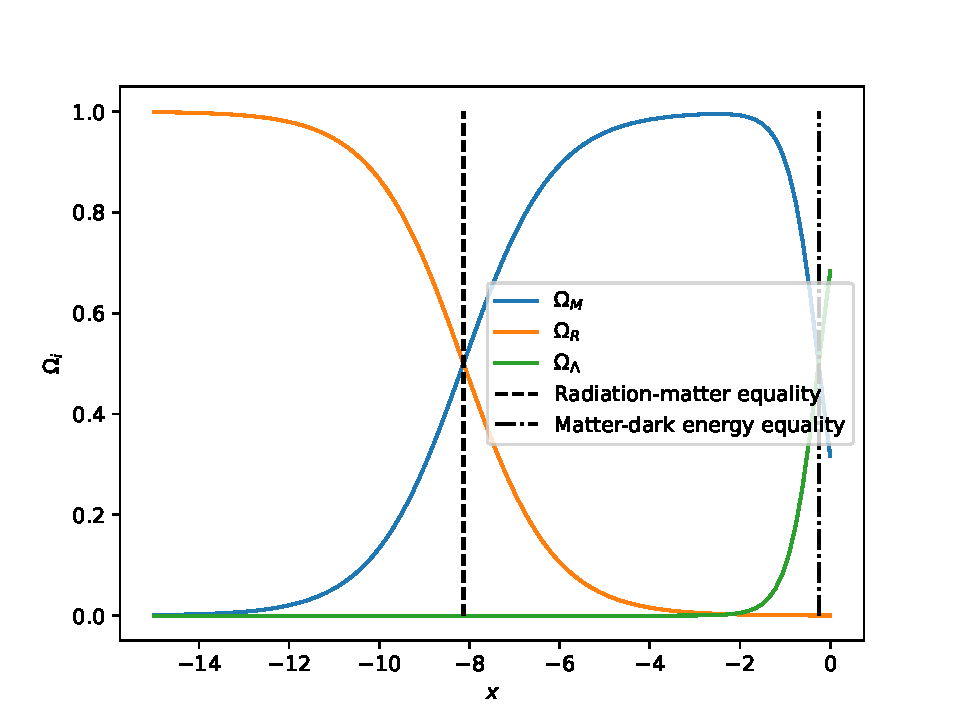
\includegraphics[width=\hsize]{figures/Omegas.pdf}
  \caption{Evolution of the densities of the components of the Universe as a function of the logarithm of the scale factor, where the density of matter, radiation and dark energy are shown, respectively, in blue, orange and green. The black vertical lines show the radiation-matter (dashed) and matter-dark energy (dot-dashed) equalities. In the beginning, radiation dominates; in between the two vertical lines, matter dominates; and, closer to today, dark energy dominates.}
     \label{fig:Omegas}
\end{figure}

\begin{figure}[ht]
\centering
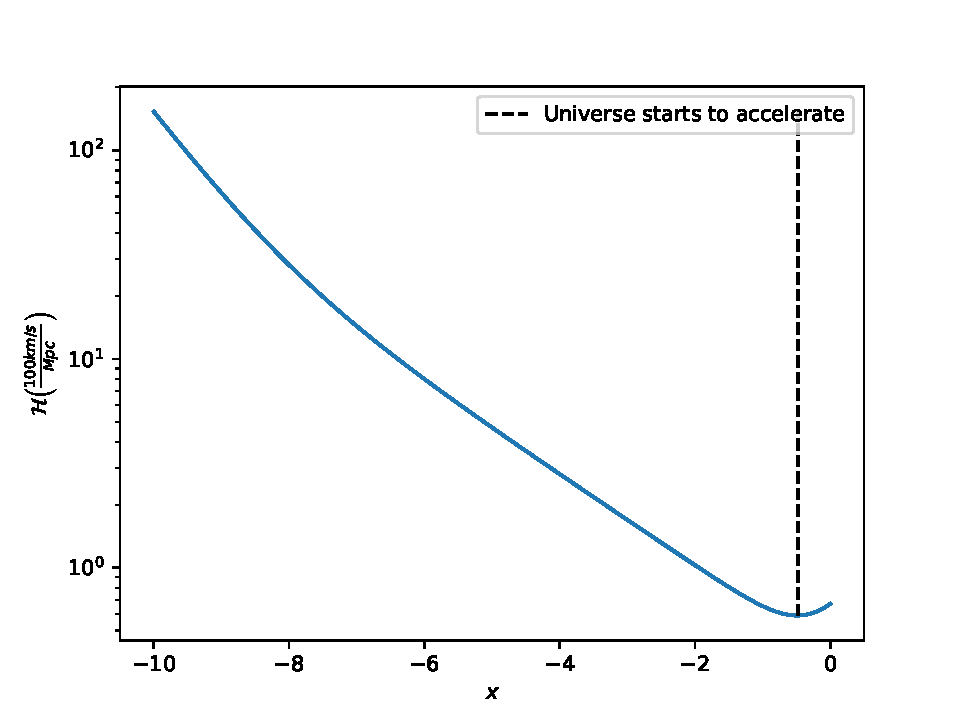
\includegraphics[width=\hsize]{figures/Hp.pdf}
  \caption{Scaled Hubble parameter as a function of the logarithm of the scale factor (blue). The black vertical dashed line represents the point where the Universe starts to accelerate.}
     \label{fig:Hp}
\end{figure}

\begin{table*}[ht]
\caption{Times of relevant events in Background Cosmology history.}             
\label{table:times}      
\centering          
\begin{tabular}{l l l l}     % 7 columns 
\hline\hline       
                      % To combine 4 columns into a single one 
& Logarithm of scale factor $x$      & Redshift $z$     & Cosmic time $t$ (Gyr)\\ 
\hline                    
Radiation-Matter Equality   & -8.1319  & 3400.3  & 5.1029 $\times 10^{-5}$ \\
Matter-Dark Energy Equality & -0.25582 & 0.29152 & 10.371                 \\
Universe starts to accelerate ($\ddot a = 0$)               & -0.47941 & 0.61513 & 7.8234\\ 
\hline                  
\end{tabular}
\end{table*}

It is also useful to look at the derivatives of $\mathcal H$ as well as the conformal time, in Figures \ref{fig:dhpdx}, \ref{fig:ddhpddx} and \ref{fig:eta}.
\begin{figure}[ht]
\centering
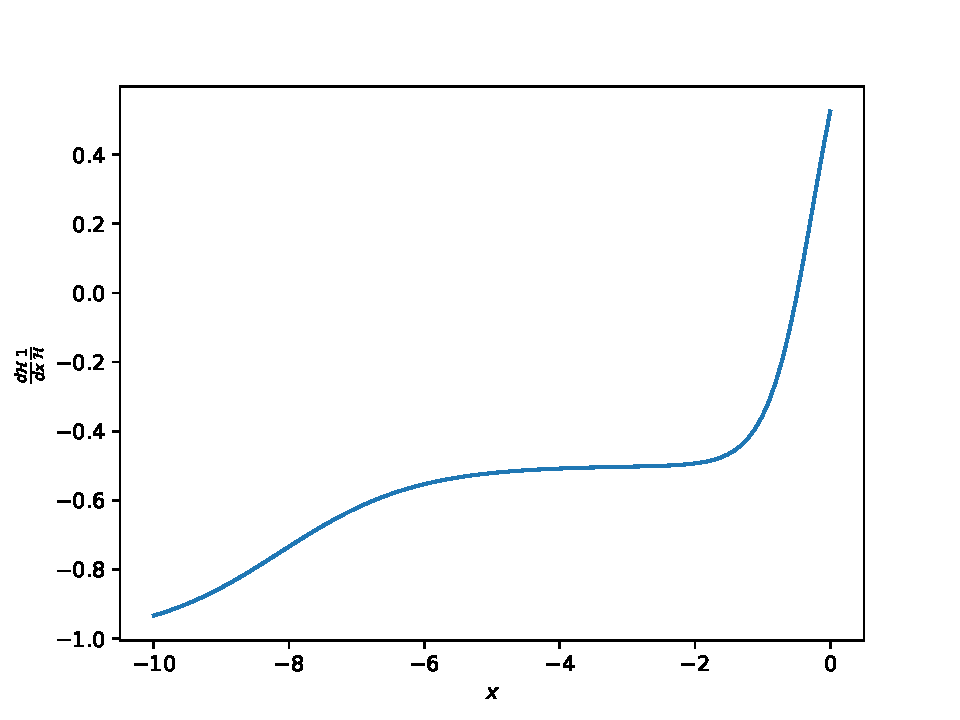
\includegraphics[width=\hsize]{figures/dHpdx_over_Hp.pdf}
  \caption{Evolution of the first derivative of the scaled Hubble parameter over the scaled Hubble parameter as a function of the logarithm of the scale factor.}
     \label{fig:dhpdx}
\end{figure}

\begin{figure}[ht]
\centering
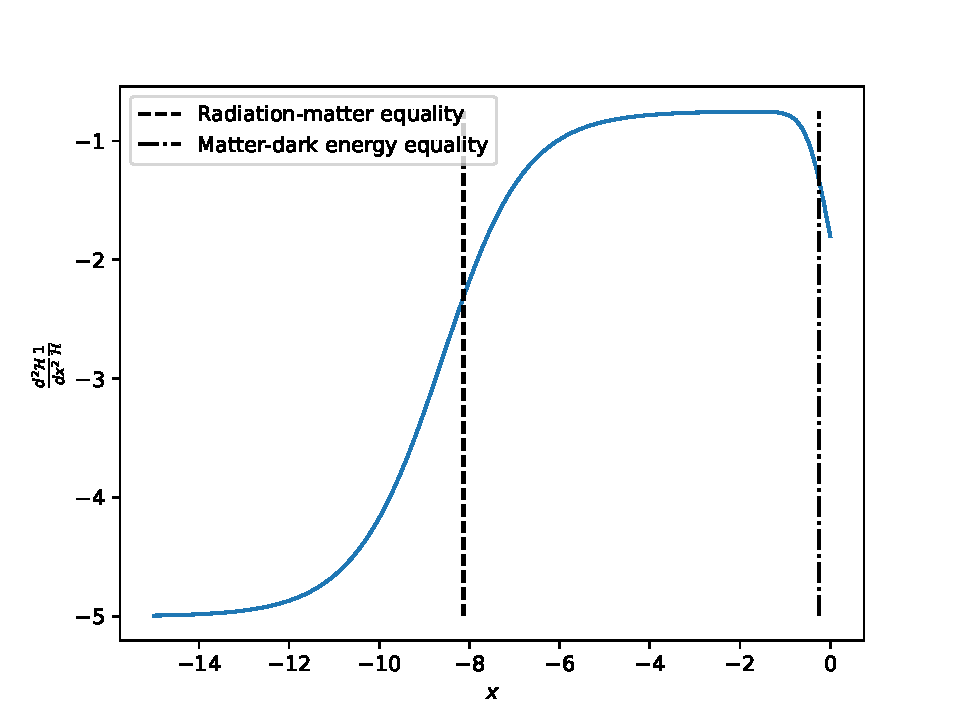
\includegraphics[width=\hsize]{figures/ddHpddx_over_Hp.pdf}
  \caption{Evolution of the second derivative of the scaled Hubble parameter over the scaled Hubble parameter as a function of the logarithm of the scale factor.}
     \label{fig:ddhpddx}
\end{figure}

\begin{figure}[ht]
\centering
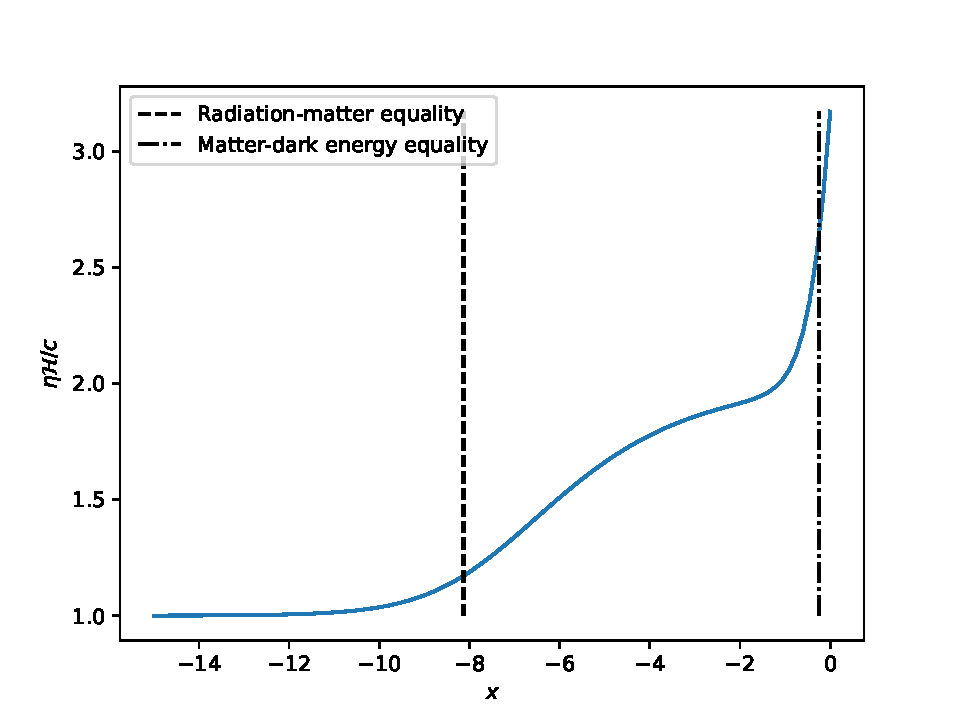
\includegraphics[width=\hsize]{figures/etaHp_over_c.pdf}
  \caption{Evolution of the conformal time times the scaled Hubble parameter as a function of the logarithm of the scale factor.}
     \label{fig:eta}
\end{figure}

As a sanity check, it is also good to look at the trends in the conformal and cosmic times in Figures \ref{fig:eta} and \ref{fig:t}. As expected, they both have an upwards trend. Additionally, we can calculate that the conformal time of today ($a = 1 \Rightarrow x = 0$) is 14.192 Gpc.

\begin{figure}[ht]
\centering
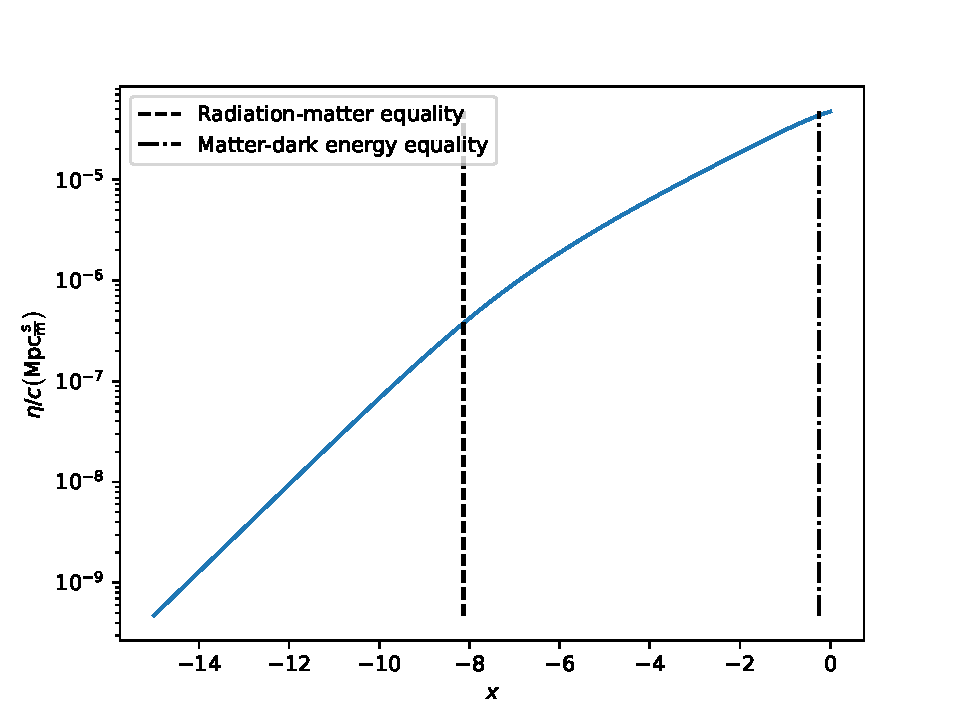
\includegraphics[width=\hsize]{figures/eta_over_c.pdf}
  \caption{Conformal time as a function of the logarithm of the scale factor.}
     \label{fig:eta}
\end{figure}

\begin{figure}[ht]
\centering
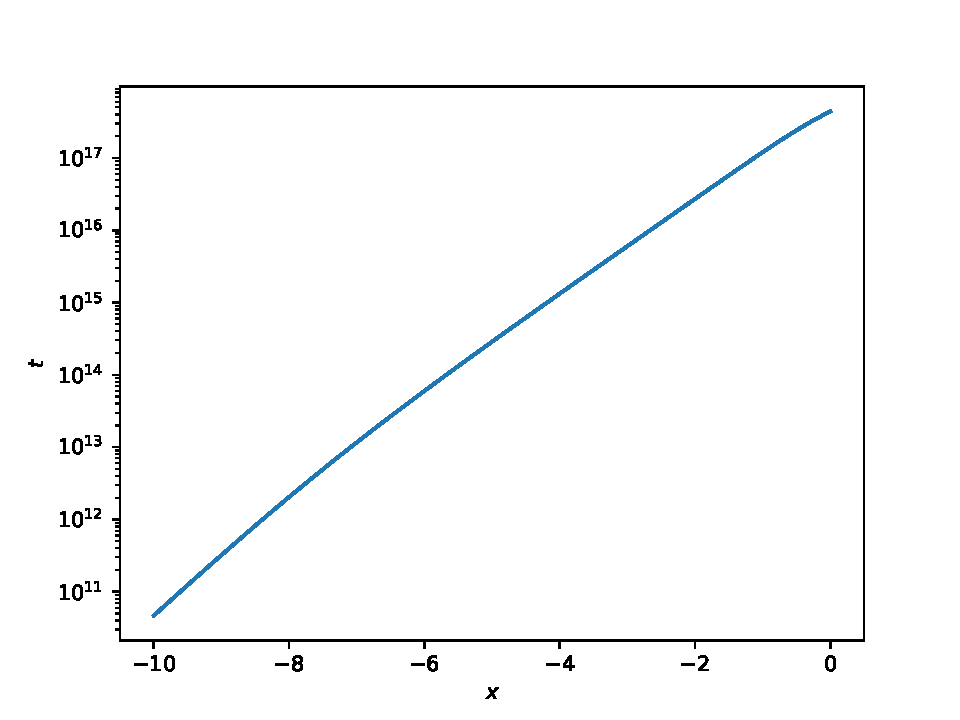
\includegraphics[width=\hsize]{figures/t.pdf}
  \caption{Cosmic time as a function of the logarithm of the scale factor.}
     \label{fig:t}
\end{figure}

An interesting result is comparing our model to the data from \cite{Betoule_2014} by looking at the luminosity distance measure in Figure \ref{fig:dL}. We see that our model has the same shape as the data, but it does not match completely, especially at lower redshifts.

\begin{figure}[ht]
\centering
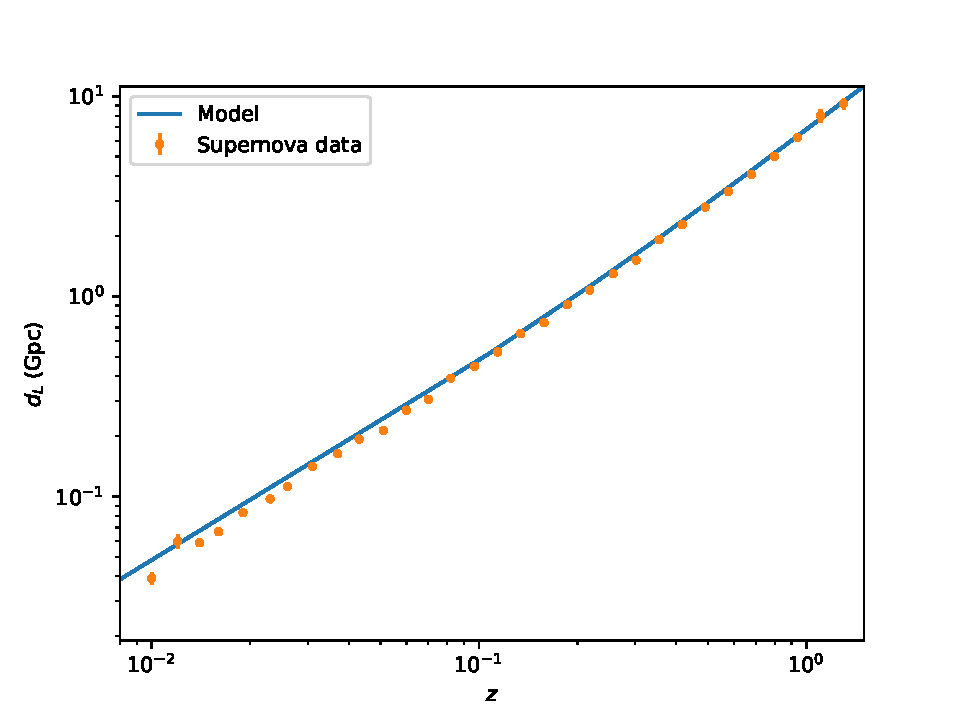
\includegraphics[width=\hsize]{figures/dL.pdf}
  \caption{Luminosity distance scaled by redshift as a function of redshift. Our model is represented as the blue curve and the data is represented as the orange circles with their respective error bars.}
     \label{fig:dL}
\end{figure}

We now want to take a look at our MCMC fits. In Figure \ref{fig:fitting}, we can see the 1$\sigma$ prediction for the value of the densities of matter and dark energy. For a flat Universe, we predict that $\Omega_M \approx0.3$ and $\Omega_\Lambda\approx0.7$. Lastly, we have a 1$\sigma$ posterior prediction for the Hubble constant as shown in Figure \ref{fit:hist} around 70 km s$^{-1}$ Mpc$^{-1}$, which does not span to the Planck best-fit value, but is within legacy results for the Hubble constant calculated by other methods.

\begin{figure}[ht]
\centering
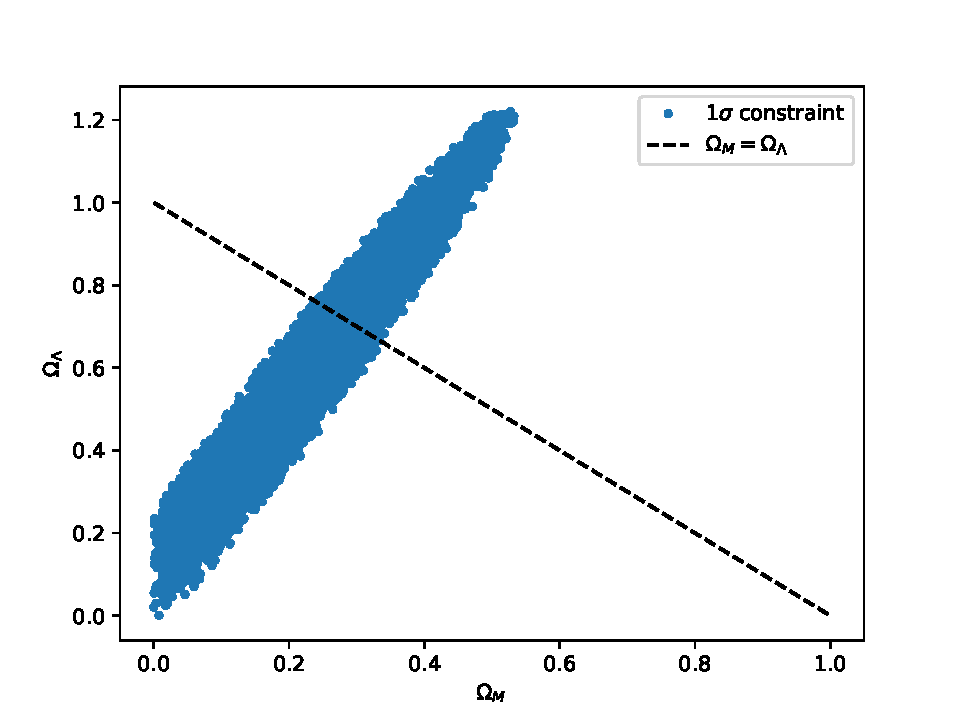
\includegraphics[width=\hsize]{figures/fitting.pdf}
  \caption{Constraints on the present-day density parameters for matter ($\Omega_M$) and dark energy ($\Omega_\Lambda$). The shaded region represents 1$\sigma$ confidence interval, indicating the most probable values for these parameters based on our MCMC fit. The black dashed line indicates where the densities would lie in a flat Universe, where, at later times, $1 = \Omega_M + \Omega_\Lambda$.}
     \label{fig:fitting}
\end{figure}

\begin{figure}[ht]
\centering
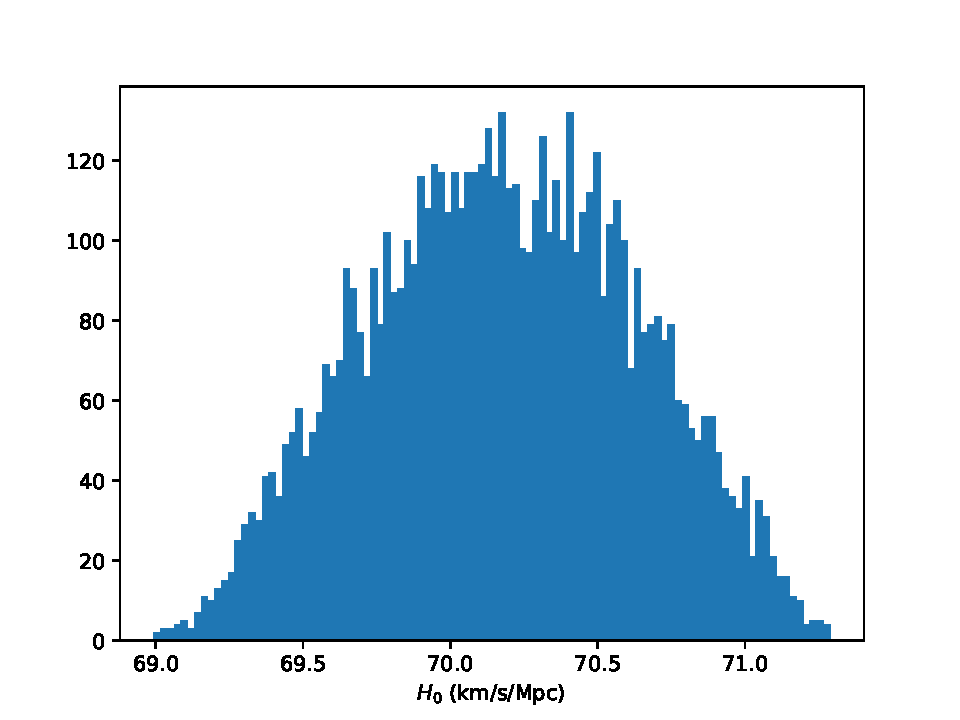
\includegraphics[width=\hsize]{figures/histogram.pdf}
  \caption{1$\sigma$ prediction for the Hubble constant.}
     \label{fit:hist}
\end{figure}

\subsection{Recombination History}

Figure \ref{fig:Xe-Saha} shows the fractional electron density $X_e$ over time $x$. The blue line describes the Saha solution. The orange line describes the full solution, starting by solving the Saha equations, until $X_e$ reaches 0.99, and then by solving the Peebles ODE. The Saha equations give a solution that falls off much faster than what is verified by experiments, and thus the need arises for the Peebles solution. Furthermore, we show the times of the last scattering and recombination, which happen almost simultaneously. Saha also predicts that recombination happens earlier than Peebles, consequence of the $X_e$ curve falling off faster. Around -8.5 to -8 and -8 to -7.5, we can see the recombination stages of singly and doubly ionised helium, following by that of hydrogen.

As we tend towards freeze-out, we can see that the fractional electron density is stable since recombination at around $0.00026736$, when ionisation is not considered.

\begin{figure}[ht]
    \centering
    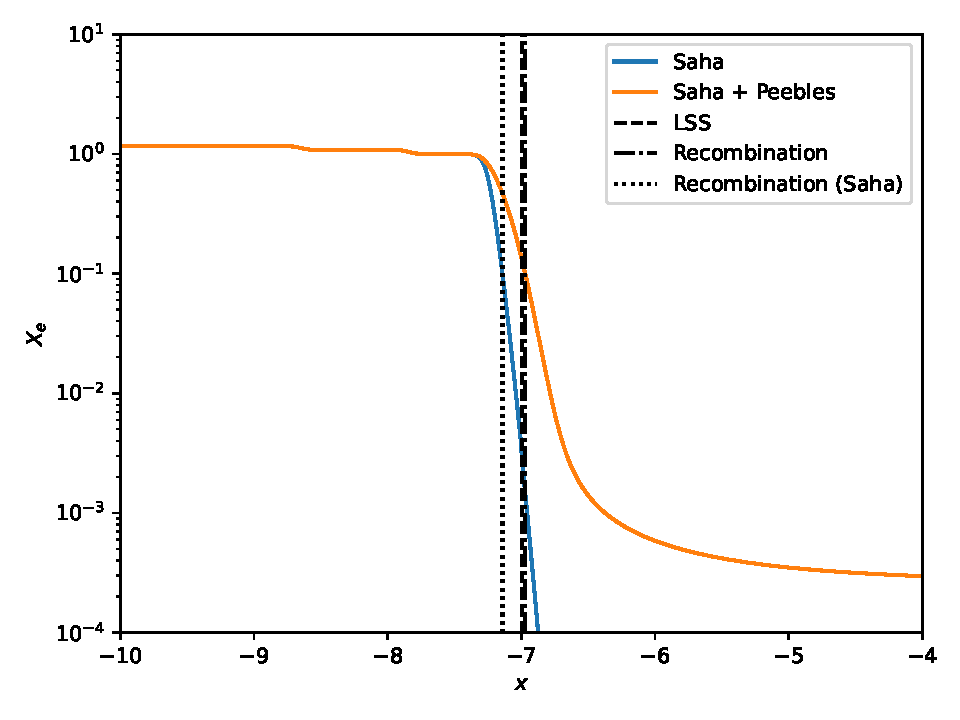
\includegraphics[width=\hsize]{report/figures/Xe.pdf}
    \caption{Fractional electron density $X_e$ given by the Saha equations (blue) and by full solution (orange) over time. Relevant times are marked in black vertical lines: the last scattering surface (surface) (LSS) (dashed),  recombination (dot-dashed) and recombination when calculated according only to the Saha equations (dotted). Reionisation is not used for the curves represented in this plot.}
    \label{fig:Xe-Saha}
\end{figure}

Calculating the fractional energy density until today, we find Figure \ref{fig:Xe-reion}. The helium recombination drop-offs are more obvious in this plot, as it is in linear scale on the y-axis, as opposed to the previous plot, which was in logarithmic scale and aimed to look at the differences between the full solution and the Saha solution. We can also see that the electron density rises again after reionization, both for hydrogen and helium. As such, we are able to identify three matter epochs: plasma (green), neutral hydrogren and helium (red) and neutral and ionised species (purple), which are separated by recombination and ionisation. These times are listed in Table \ref{table:times-rec}.

\begin{figure}[ht]
    \centering
    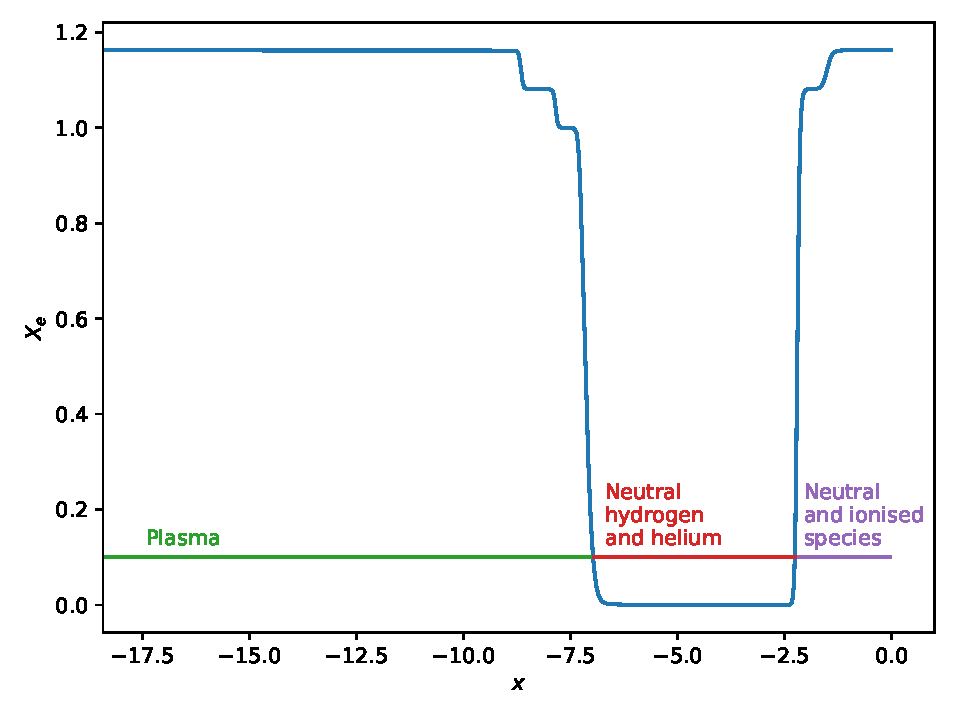
\includegraphics[width=\hsize]{report/figures/Xe-reion.pdf}
    \caption{Fractional electron density $X_e$ (blue) over time. The dominating matter epochs are shown by the horizontal lines: plasma (green) dominates in the early Universe, neutral hydrogen and helium (red) dominate after recombination and before reionization, and a mixture of neutral and ionised species (purple) dominate after reionization.}
    \label{fig:Xe-reion}
\end{figure}

\begin{table*}[ht]
\caption{Times of relevant events in recombination history.}             
\label{table:times-rec}      
\centering          
\begin{tabular}{l l l l}     % 7 columns 
\hline\hline       
                      % To combine 4 columns into a single one 
& Logarithm of scale factor $x$      & Redshift $z$     & Cosmic time $t$ (Myr)\\ 
\hline                    
Last scattering   & -6.9901  & 1084.8  & 0.37478 \\
Recombination & -6.9701 & 1063.3 & 0.38758                 \\
Recombination (according to Saha) & -7.1403 & 1260.9 & 0.29069\\
\hline                  
\end{tabular}
\end{table*}

The optical depth $\tau$ (blue) and its first (orange, times -1) and second (green) derivatives w.r.t. $x$ over time $x$ are shown in Figure \ref{fig:tau}. We can see that the optical depth in the early Universe is very large, meaning the photon-baryon plasma is an optically thick medium, where no light can be transmitted. The time of the last scattering is pointed out by the black vertical dashed line, defined by $\tau=1$. After this point, the optical depth is lower than one stable until reionisation, and thereafter it starts decreasing again, meaning photons are able to travel through the medium since recombination until today.

\begin{figure}[ht]
    \centering
    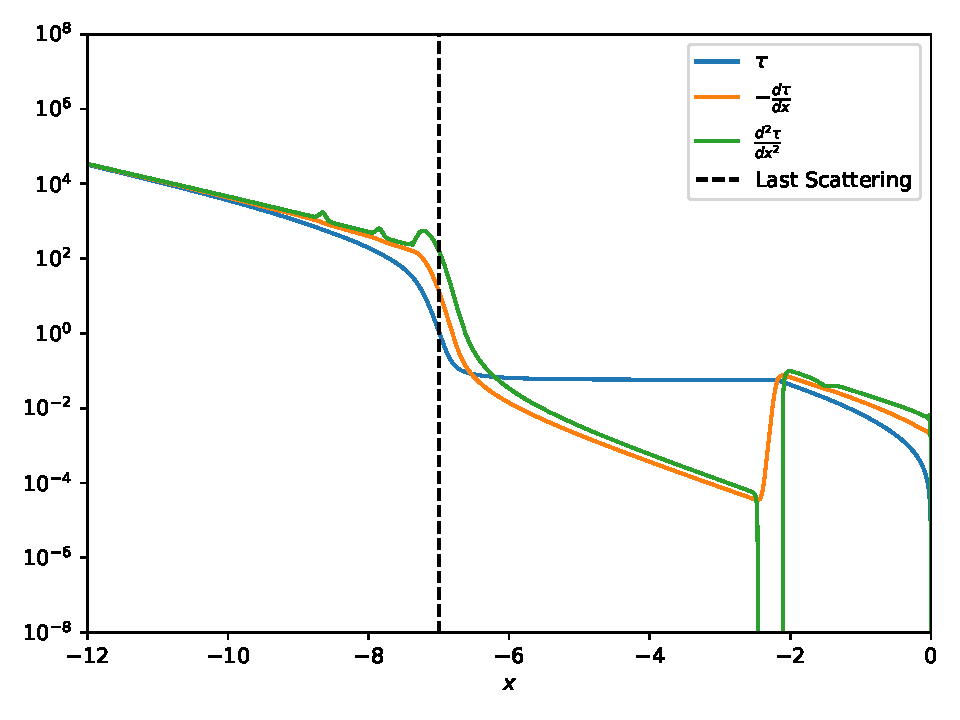
\includegraphics[width=\hsize]{report/figures/tau.pdf}
    \caption{Optical depth $\tau$ (blue), as well as its first (orange) and second (green) derivatives w.r.t. $x$ over time. The time of the last scattering is pointed out by the black vertical dashed line.}
    \label{fig:tau}
\end{figure}

One last useful visualization is Figure \ref{fig:gtilde}, where we look at the visibility function $\tilde g$ (blue) and its first (orange) and second (green) derivatives w.r.t. $x$ over $x$, with each curve normalized. $\tilde g$ peaks around the same time as recombination, and then there is a smaller peak around reionisation.

\begin{figure}[ht]
    \centering
    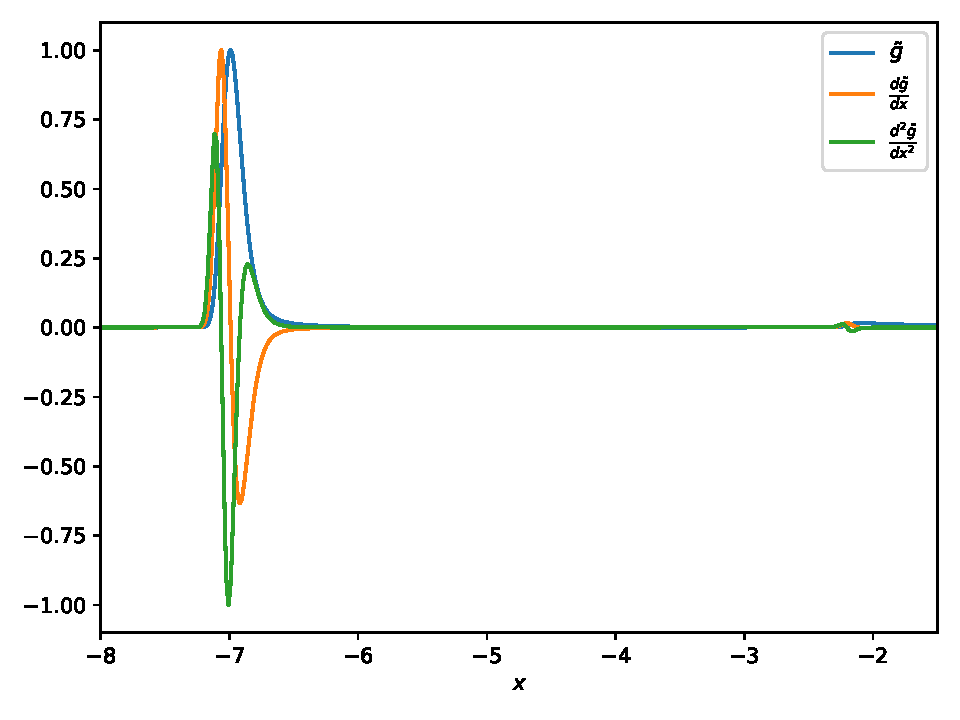
\includegraphics[width=\hsize]{report/figures/gtilde.pdf}
    \caption{Visibility function $\tilde g$ (blue) and its first (orange) and second (green) derivatives, peak normalised, w.r.t. $x$ over time.}
    \label{fig:gtilde}
\end{figure}

We can calculate the distance a sound-wave can propagate through the photon-baryon plasma from the Big Bang until recombination by calculating the sound-horizon at decoupling, which is then $r_s = 144.84$ Mpc.

\subsection{Perturbations}

Let us now take a look at how our quantities of interest evolve with time.

First, we look at the density perturbations in Figure \ref{fig:densities}. In all of the panels, we can see that the quantities are constant up until a certain time. Each scale starts diverging from this constant value at a different time, the time each of them entering the horizon, with the smallest scale, naturally, being the first to enter the horizon and be able to interact gravitationally. Once inside the horizon, pressure and gravitational forces come into play. The photon and neutrino overdensities begin to oscillate due to this interplay: gravitational attraction causes overdensities to grow, while radiation pressure resists compression, producing acoustic oscillations. These oscillations are gradually dampened by the Universe’s expansion. The amplitude and behavior of these oscillations vary by scale, with smaller scales exhibiting more rapid and earlier oscillations. CDM, on the other hand, does not interact, and thus does not go through these oscillations. For baryons, the same oscillatory behavior happens, as, before recombination, baryons are tightly coupled to photons through Thomson scattering, forming a photon-baryon fluid. After recombination, baryons are no longer supported by radiation pressure and instead begin to fall into the gravitational potential wells formed by CDM clusters.

\begin{figure*}[ht]
  \centering
  \subfigure[]{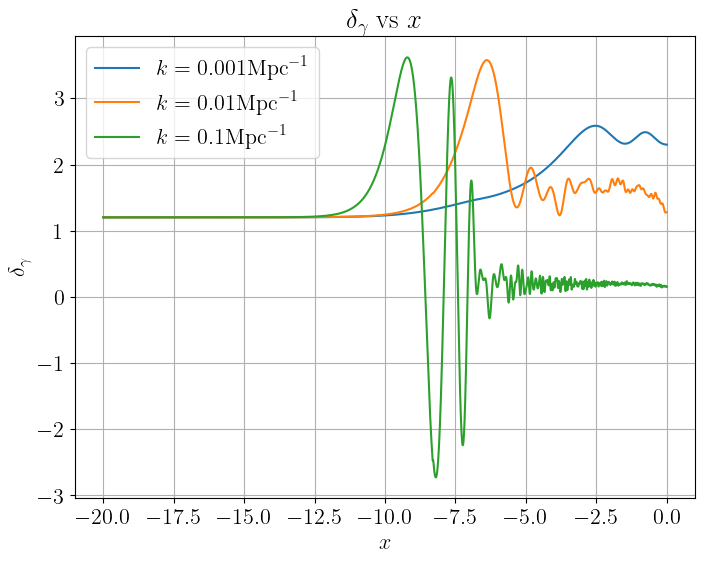
\includegraphics[width=0.32\hsize]{report/figures/delta_gamma.png}}\quad
  \subfigure[]{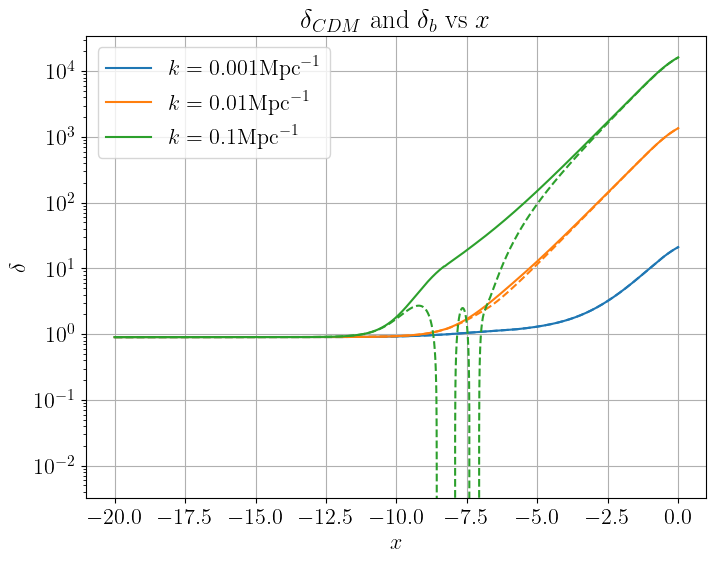
\includegraphics[width=0.32\hsize]{report/figures/delta_cdm_delta_b.png}}\quad
  \subfigure[]{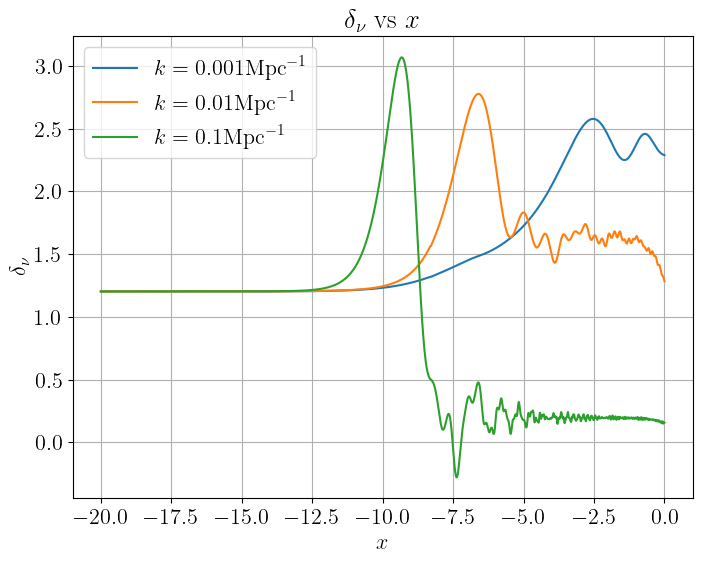
\includegraphics[width=0.32\hsize
]{report/figures/delta_nu.png}}
\caption{Density perturbations $\delta$ over time. Each panel shows the evolution of the photon overdensity (a), CDM (solid) and baryon (dashed) overdensity (b) and neutrino overdensity (c). Each of the colored curves shows a different scale from biggest ($k = 0.001$ Mpc$^{-1}$, blue) to smallest ($k=0.1$ Mpc$^{-1}$, green). \hw{Fig 16b,17b. Minor thing: Maybe use | delta$_b$ |, | v$_b$ | so that one sees the missing oscillations (where these things are negative).}}
\label{fig:densities}
\end{figure*}

The evolution of the perturbation velocities is shown in Figure \ref{fig:velocities} and the shape of the curves is explained by the same physics. Photons and neutrinos exhibit oscillatory velocity perturbations, just like their density counterparts. CDM, lacking pressure support, exhibits little oscillatory behavior, while baryons again follow the photons prior to recombination due to tight coupling, and afterward begin to follow CDM.

\begin{figure*}[ht]
  \centering
  \subfigure[]{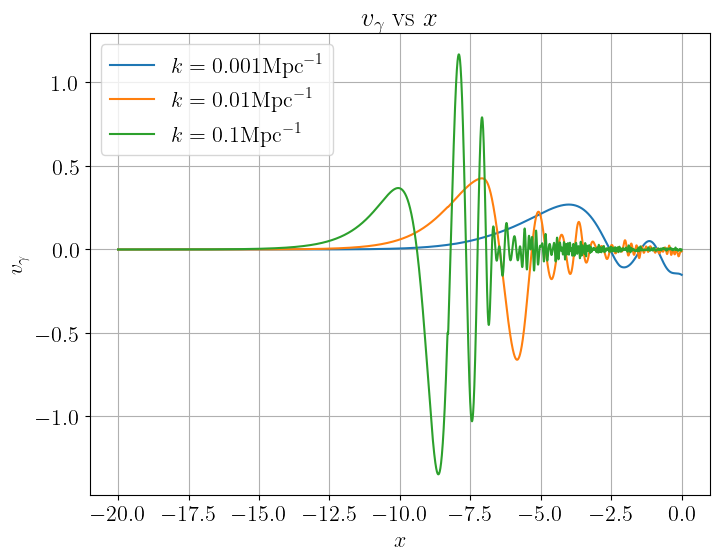
\includegraphics[width=0.32\hsize]{report/figures/v_gamma.png}}\quad
  \subfigure[]{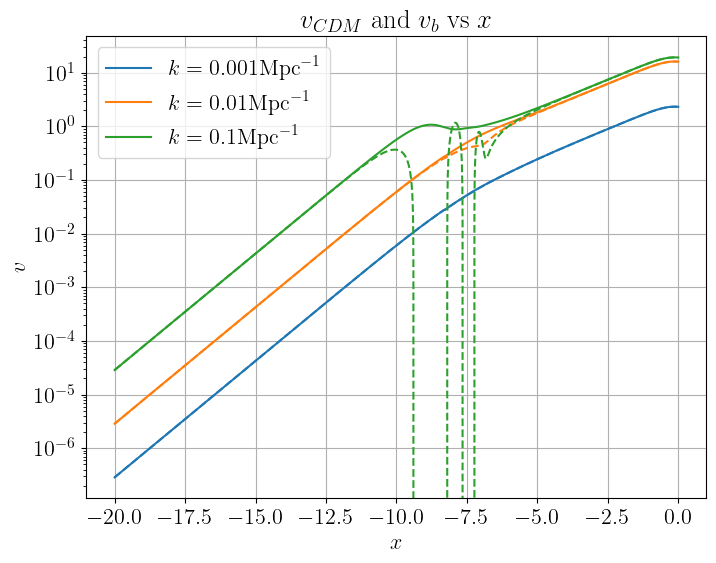
\includegraphics[width=0.32\hsize]{report/figures/v_cdm_v_b.png}}\quad
  \subfigure[]{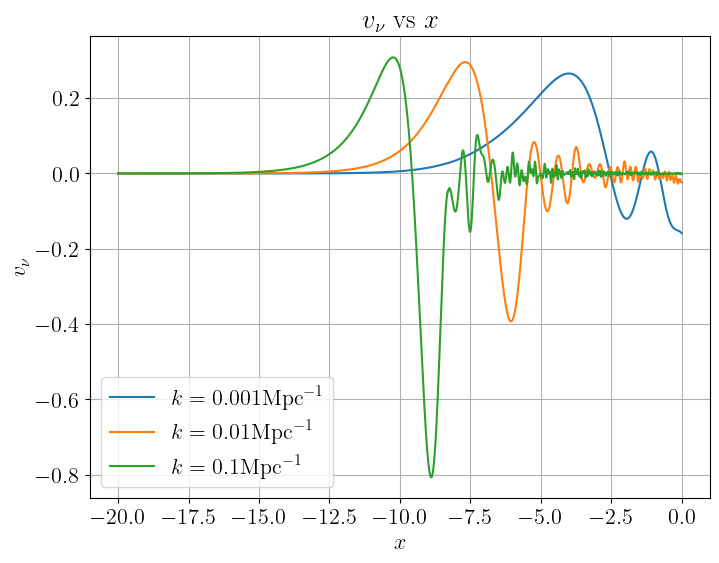
\includegraphics[width=0.32\hsize
]{report/figures/v_nu.png}}
\caption{Velocity perturbations $v$ over time. Each panel shows the evolution of the photon perturbation velocity (a), CDM (solid) and baryon (dashed) perturbations velocity (b) and neutrino perturbation velocity (c). Each of the colored curves shows a different scale from biggest ($k = 0.001$ Mpc$^{-1}$, blue) to smallest ($k=0.1$ Mpc$^{-1}$, green).}
\label{fig:velocities}
\end{figure*}

Figure \ref{fig:theta2-nu2} shows the evolution of the photon and neutrino quadrupoles, which, once again, can be largely explained by the same physics. The photon quadrupole, however, has a slightly different behavior than described before, as the modes all start oscillating at the same time, once photons decouple, as before that, frequent Thomson scattering suppresses higher moments. Neutrinos, which decouple much earlier, begin developing a quadrupole much sooner.

\begin{figure}[ht]
    \centering
    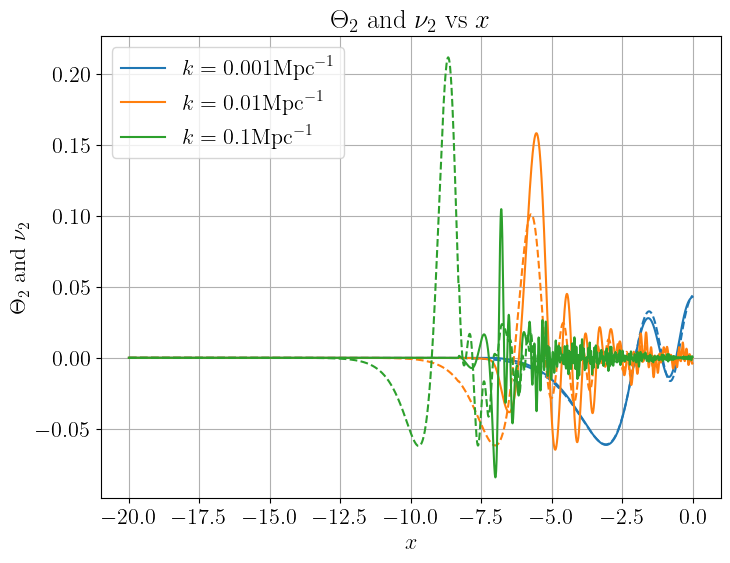
\includegraphics[width=\hsize]{report/figures/Theta2_Nu2.png}
    \caption{Photon (solid) and neutrino (dashed) quadrupoles over time. Each of the colored curves shows a different scale from biggest ($k = 0.001$ Mpc$^{-1}$, blue) to smallest ($k=0.1$ Mpc$^{-1}$, green).}
    \label{fig:theta2-nu2}
\end{figure}

Figure \ref{fig:potentials} shows the evolution of the metric potentials $\Phi$, as well as the anisotropic stress ($\Phi +\Psi$) over time. It is particularly interesting to look at the anisotropic stress (dashed) curve, where we see that the approximation $\Phi = - \Psi$ holds at later times, when the photon and neutrino quadrupoles are negligible (seen when compared to Figure \ref{fig:theta2-nu2}), i.e. stress from different directions is only relevant when photons and neutrinos have appreciable quadrupole momentums.

\begin{figure}[ht]
    \centering
    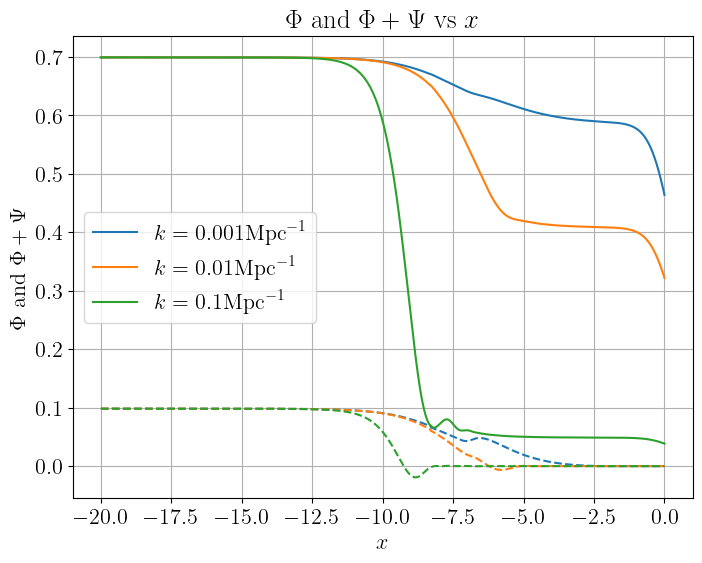
\includegraphics[width=\hsize]{report/figures/Phi_Psi.png}
    \caption{$\Phi$ potential (solid) and anisotropic stress (dashed) over time. Each of the colored curves shows a different scale from biggest ($k = 0.001$ Mpc$^{-1}$, blue) to smallest ($k=0.1$ Mpc$^{-1}$, green).}
    \label{fig:potentials}
\end{figure}

Lastly, we take a look at how polarization evolves over time in Figure \ref{fig:thetap}. The same dampened oscillatory behavior is present as in the temperature perturbations, but here we can see that the scale is irrelevant for when the modes start oscillating, as polarization is only relevant after photons decouple, as similarly seen for the temperature quadrupole.

\begin{figure*}[ht]
    \centering
    \subfigure[]{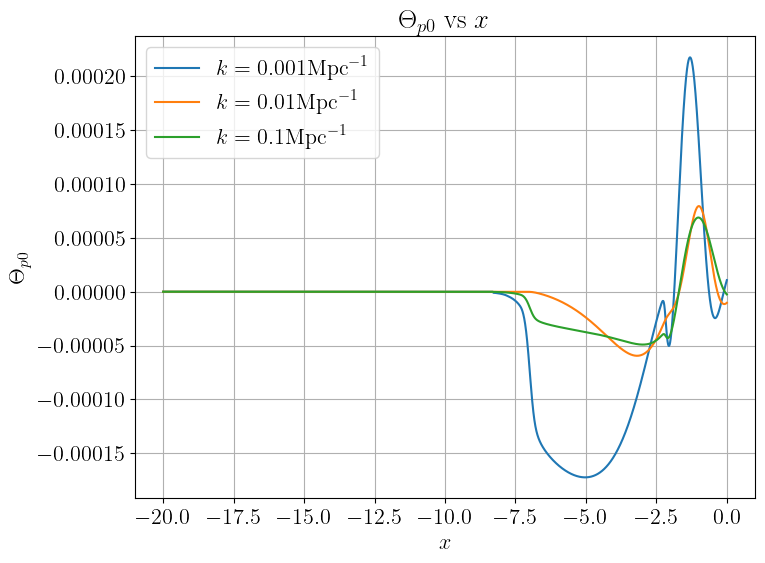
\includegraphics[width=0.32\hsize]{report/figures/Theta_p0.png}}\quad
    \subfigure[]{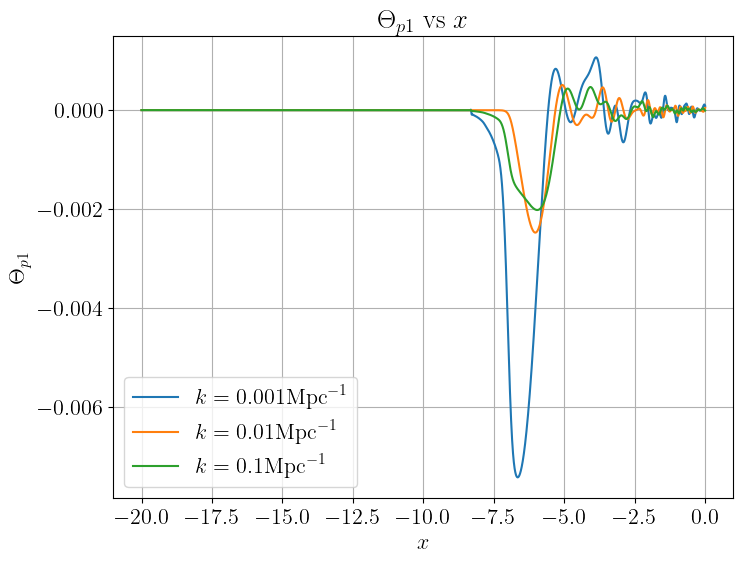
\includegraphics[width=0.32\hsize]{report/figures/Theta_p1.png}}\quad
    \subfigure[]{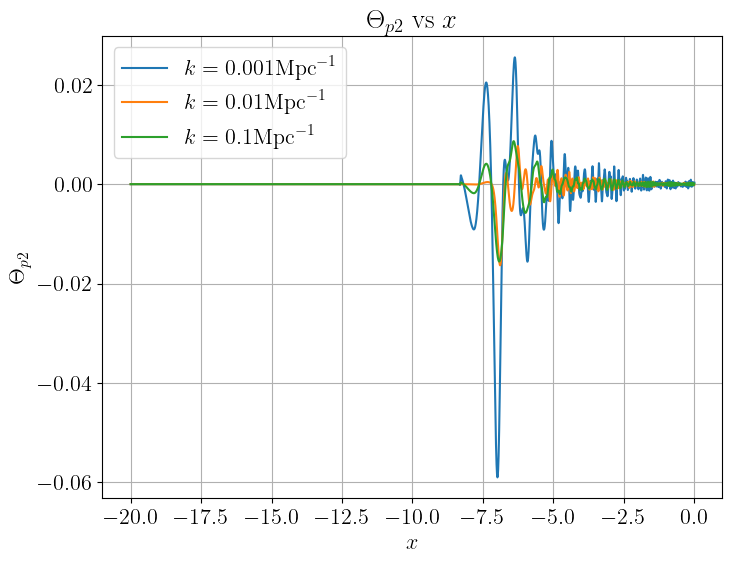
\includegraphics[width=0.32\hsize]{report/figures/Theta_p2.png}}
    \caption{Photon monopole (a), dipole (b) and quadrupole polarization perturbations over time. Each of the colored curves shows a different scale from biggest ($k = 0.001$ Mpc$^{-1}$, blue) to smallest ($k=0.1$ Mpc$^{-1}$, green).}
    \label{fig:thetap}
\end{figure*}

\subsection{Power Spectrum}

Let us first take a look at what $\Theta_l$ that we generated via line of sight integration look like in Figure \ref{fig:thetaell}, where the $x$-axis is presented in unitless coordinates $k\eta_0$. We see the oscillations introduced by the spherical Bessel functions $j_\ell$, which start only when $\ell\sim k\eta_0$ (in particular, we see that the curve for $\ell=1000$ does not even start oscillating within the limits we are looking at), used as a consistency check.

\begin{figure}[ht]
    \centering
    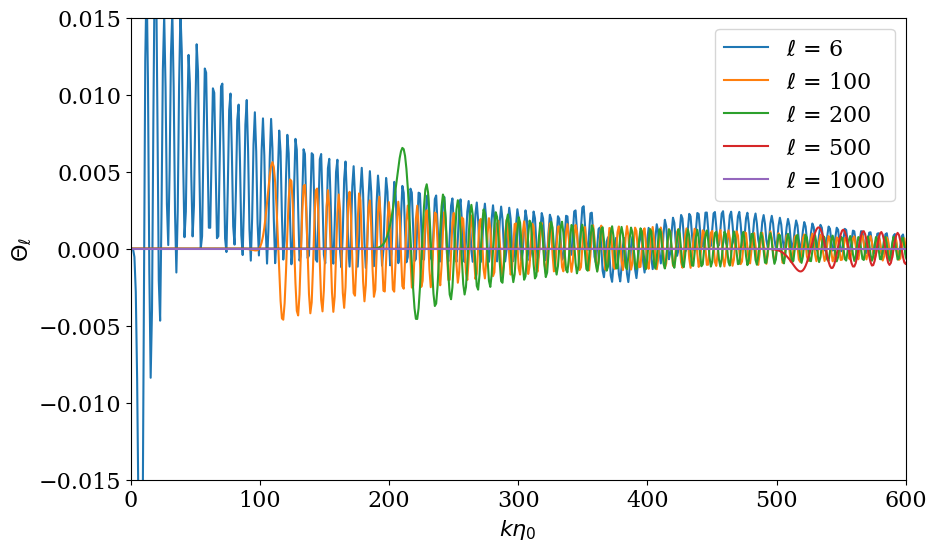
\includegraphics[width=\linewidth]{report/figures/theta_ell_of_k.png}
    \caption{Photon multipoles $\Theta_\ell$ for different $\ell$s (respectively, 6, 100, 200, 500 and 1000 in blue, orange, green, red and purple) over wavenumber multiplied by the conformal time today $k\eta_0$.}
    \label{fig:thetaell}
\end{figure}

We see a similar oscillatory pattern when looking at the full integrand for $C_\ell$, $\Theta_\ell^2/k$, plotted in Figure \ref{fig:integrand}, where the oscillations also start around $\ell\sim k\eta_0$.

\begin{figure}[ht]
    \centering
    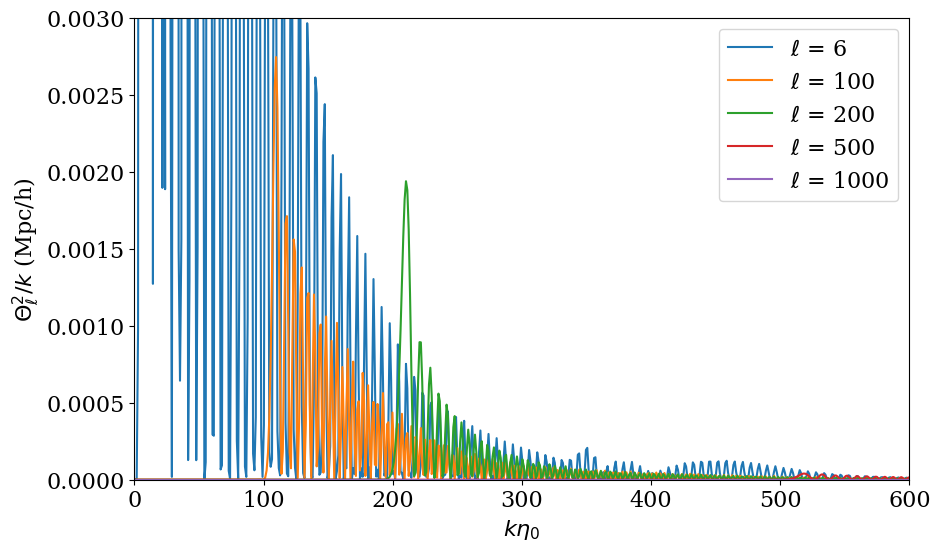
\includegraphics[width=\linewidth]{report/figures/theta_ell2_of_k.png}
    \caption{Integrand of $C_\ell$, $\Theta_\ell^2/k$, for different $\ell$s (respectively, 6, 100, 200, 500 and 1000 in blue, orange, green, red and purple) over wavenumber multiplied by the conformal time today $k\eta_0$.}
    \label{fig:integrand}
\end{figure}

Finally, we can go over the main results of the present paper: the simulated power spectra compared to observations, as well as maps of the sky. We start by presenting the CMB temperature power spectrum in Figure \ref{fig:ps-tt}. The power spectrum is presented as $\frac{\ell(\ell+1)C_\ell^\text{TT}}{2\pi}$ in order to evidence the low-$\ell$ plateau. We can see that our simulations and the data agree well. It is now interesting to look at what each feature in the power spectrum means physically.

\begin{figure}[ht]
    \centering
    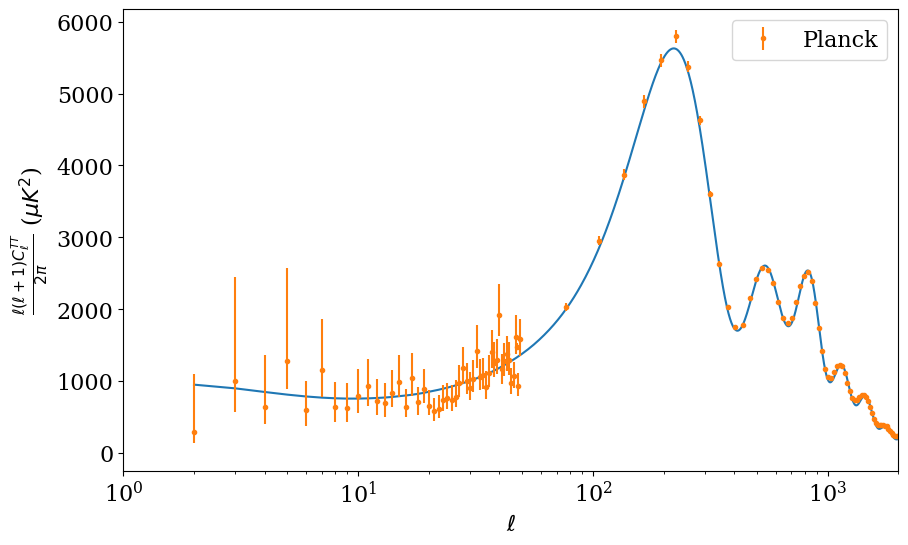
\includegraphics[width=\linewidth]{report/figures/power_spectrum_TT.png}
    \caption{CMB temperature power spectrum. The theoretical curve is presented in blue and observations from \cite{2020} are presented in orange with their respective error bars. The power spectrum is presented as $\frac{\ell(\ell+1)C_\ell^\text{TT}}{2\pi}$ and the $x$-axis is in logscale in order to evidence the low-$\ell$ plateau.}
    \label{fig:ps-tt}
\end{figure}

Starting at the low-$\ell$s, we can observe there is a plateau until around $\ell\sim20$, called the Sachs-Wolfe plateau, because we can approximate the photon multipole equation by the first term. We see it as a plateau because the spectral index $n_s$ used for our simulations (and measured in experiments) is very close to one ($n_s=0.965$). If we look closely, we can actually tell that it tilts slightly up at lower $\ell$s, as $n_s$ is smaller than one. However, as we can also tell by the large error bars, there is a large uncertainty in this regime, called the cosmic variance. This happens because large-scale measurements are affected by measurement position, and we are limited by where we can make measurements in.

The Sachs-Wolfe plateau is followed by a peak at around $\ell\sim 200$. The position of this peak in a flat Universe is determined by
\begin{equation}
\ell \sim \pi \frac{\eta_0 - \eta_{\rm rec}}{r_s},
\end{equation}
meaning it depends on the sound horizon at decoupling $r_s$ and the angular diameter distance $D_A(a_\text{rec}) = \frac{\eta_0-\eta_\text{rec}}{a_\text{rec}}$, which, themselves depend, respectively, on baryon density, which affects sound speed, and (mainly or most illustratively) on curvature, as adding curvature to the model makes the spots in the CMB appear larger or smaller than they would be at flat space.

As for the amplitudes of the peaks in the spectrum (most significantly, the first, second and third ones) and specifically their relative amplitudes, the most significant contributers are the baryon $\Omega_{b0}h^2$ and matter $\Omega_{M0}h^2$ densities. A higher baryon density will lead to a more significant baryon loading effect, which implies that $\Theta_\ell$ will not oscillate around zero (which can already be seen in Figure \ref{fig:thetaell}), but instead a negative term is added. Consequently, the even peaks (where the $\cos$ term in the spherical Bessel functions is positive) will be dampened and the odd peaks (where the same term is negative) will be enhanced). On the other hand, increasing matter density will decrease the radiation driving effect. This effect is caused by modes that enter the horizon during the radiation-dominated era, where gravitational potentials decay since radiation cannot cluster fast enough to fight the expansion of the Universe. As such, modes start oscillating, but then stop, as there is no significant gravitational potential, and thus the amplitude increases. With higher matter density, there is more gravity and thus potentials decay slower, damping the amplitude.

A last big defining feature of the CMB power spectrum is the so-called damping tail at $\ell\gtrsim800$. This feature is mainly affected by the diffusion damping effect. A photon moves $\lambda = \frac{1}{n_e\sigma_T}$ in between scattering from baryons and it scatters $N = \frac{n_e\sigma_T}{H}$ times in one Hubble time $H^{-1}$. As such, a photon on a random walk will, on average, travel, in one Hubble time,
\begin{equation} \label{eq:diffusion-length}
D = \frac{1}{n_e\sigma_T} \cdot \sqrt{\frac{n_e\sigma_T}{H}}.
\end{equation}
Perturbations at scales smaller than $D$ are negligible and simply seen as diffusing photons. Decreasing baryon density decreases the amount of free electrons, which we can see directly from \eqref{eq:diffusion-length}, increases the diffusion length, thus increasing damping. Similarly, increasing matter density increases the expansion rate at recombination, decreasing $H$ and thus increasing the diffusion length and consequently damping the diffusion tail.

We enumerated the most defining features of the CMB power spectrum and what affects them the most, but it is also worth mentioning some other parameters that have more general effects on it:
\begin{itemize}
    \item The primordial amplitude $A_s$, which sets the amplitude of the initial perturbation and thus sets the amplitude of the whole spectrum.
    \item The optical depth at reionization $\tau_\text{reion}$, which is highly degenerate with $A_s$, since it also affects the overall amplitude of the spectrum as $C_\ell \propto e^{-2\tau_\text{reion}}$, except for the largest scales (lowest $\ell$s), which correspond to the modes that only enter the horizon very close to today.
    \item Curvature $\Omega_{k0}$, which, other than its main effect, which is shifting the peaks, will also affect the tilt of the Sachs-Wolfe plateau.
    \item Dark energy density parameter $\Omega_{\Lambda0}$, which changes the distance to the surface of last scattering, as adding more dark energy means its repulsive force will cause the Universe to expand faster. As such, the position of the peaks will be slightly influenced, as well as the tilt on the Sachs-Wolfe plateau.
    %\item The number of effective degrees of freedom $N_\text{eff}$, which, when increased, increases the expansion rate at recombination
    \item The primordial helium abundance $Y_p$, which, when increased, decreased the number of free electrons, increasing the diffusion length and thus further damping the tail.
\end{itemize}

Next, we can look at the CMB polarization power spectrum, as well as the temperature-polarization cross-spectrum, compared to the temperature power spectrum in Figure \ref{fig:power-spectra}. Once again, we can see that our simulations agree with the observations, further supporting that our model and parameters are fairly well-chosen. However, in this figure it is more obvious that there seems to be a slight mismatch in the peak position, which, as we went over, might indicate that we should have used slightly different values for $\Omega_{K}$ or $\Omega_\Lambda$.

\begin{figure}
  \centering
  \begin{tabular}{@{}c@{}}
    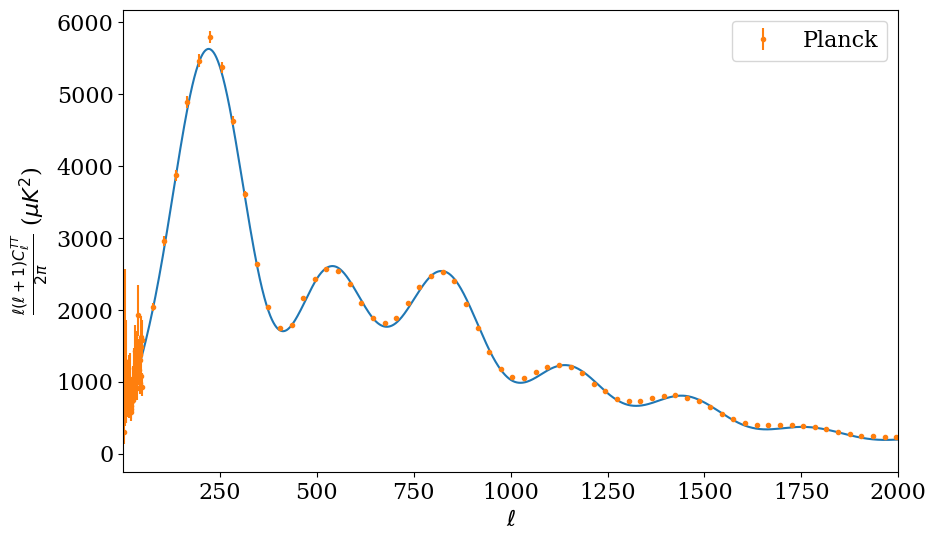
\includegraphics[width=\linewidth]{report/figures/power_spectrum_TT_linear.png} \\[\abovecaptionskip]
    \small (a)
  \end{tabular}

  \vspace{\floatsep}
  \begin{tabular}{@{}c@{}}
       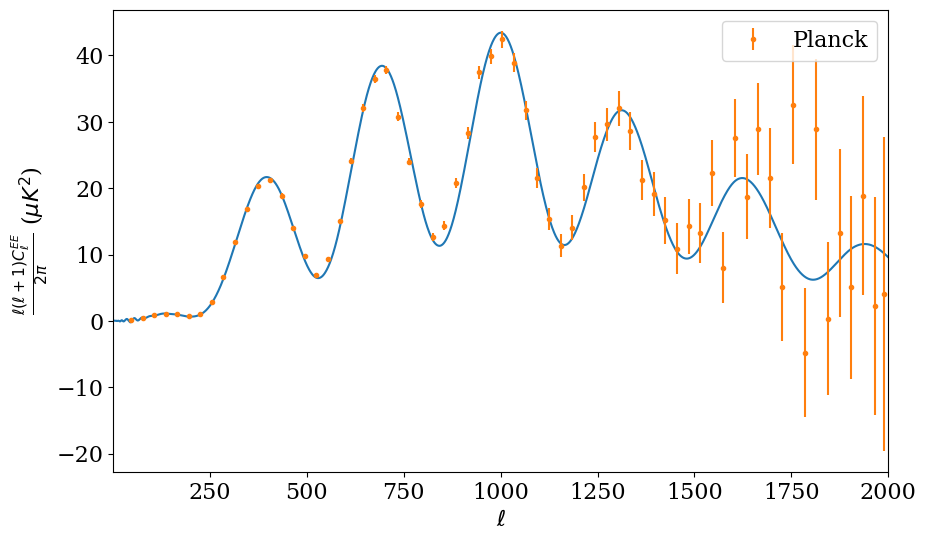
\includegraphics[width=\linewidth]{report/figures/power_spectrum_EE.png} \\[\abovecaptionskip]
    \small (b)
  \end{tabular}


  \vspace{\floatsep}

  \begin{tabular}{@{}c@{}}
    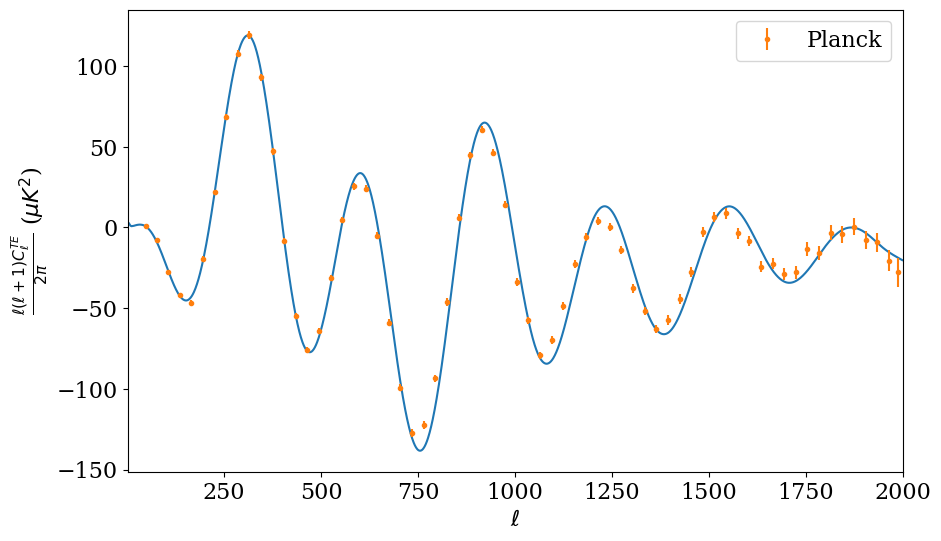
\includegraphics[width=\linewidth]{report/figures/power_spectrum_TE.png} \\[\abovecaptionskip]
    \small (c)
  \end{tabular}

  \caption{CMB temperature (a) and E-mode polarization power spectra (b) and temperature-polarization cross spectrum (c). The theoretical curve is presented in blue and observations from \cite{2020} are presented in orange with their respective error bars. The power spectra are presented as $\frac{\ell(\ell+1)C_\ell^\text{TT}}{2\pi}$.}\label{fig:power-spectra}
\end{figure}

The leading contribution for the polarization power spectrum is that of the photon quadrupole, whereas for the temperature one it is the monopole. These two are out of phase, meaning, where the temperature power spectrum has peaks, the polarization one will have dips and vice-versa, which we can confirm from the figure. Perhaps more interestingly, we know that polarization is not only generated at last scattering, but also during reionization, which translates into a small "bump" at small $\ell$s in the E-mode polarization spectrum, whose amplitude is $\propto \tau_{\rm reion}^2$, and which is a brilliant way of breaking the $\tau_\text{reion}$ degeneracies with $A_s$.

From this, we can simulate what the CMB anisotropies look like at a Universe with a random field as initial conditions, and this is shown in Figure \ref{fig:cmb-map}.

\begin{figure}[ht]
    \centering
    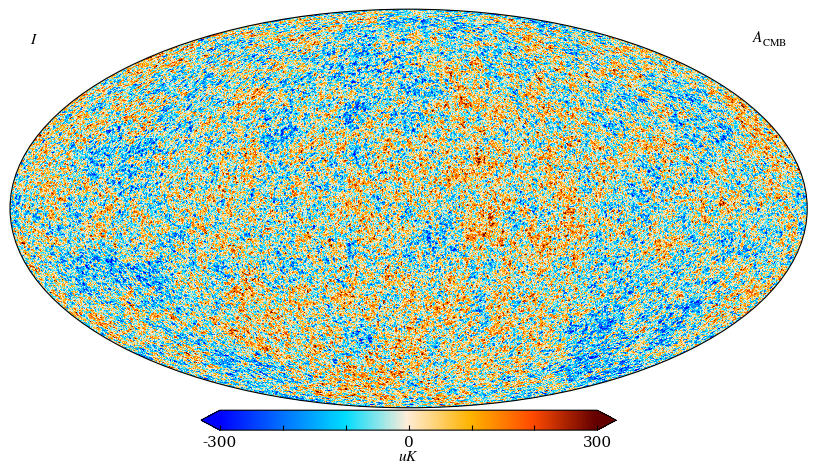
\includegraphics[width=\linewidth]{report/figures/cmb_map_TT.png}
    \caption{Temperature CMB map.}
    \label{fig:cmb-map}
\end{figure}

Even though we can see that some defining features that exist in the CMB in our Universe are not there (such as the cold spot), the map looks reasonable, with temperatures in the same order as \cite{2020}, and smaller hot and cold spots.

Lastly, we can take a look at the matter power spectrum in Figure \ref{fig:ps-matter}.

\begin{figure}[ht]
    \centering
    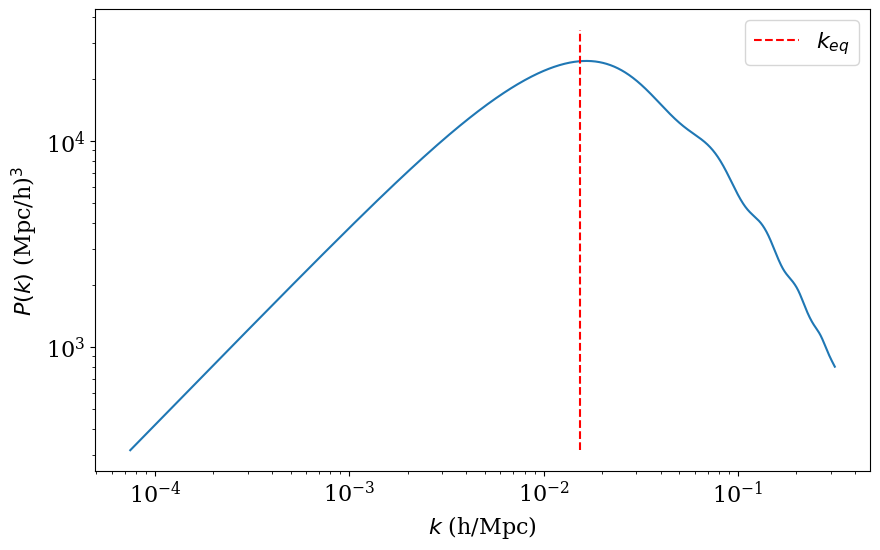
\includegraphics[width=\linewidth]{report/figures/matter_power_spectrum.png}
    \caption{Matter power spectrum $P(k)$ over wavenumber $k$ (blue) in a log-log plot. The red dashed line marks the wavenumber determined by the scale factor at matter-radiation equality.}
    \label{fig:ps-matter}
\end{figure}

The general shape of the curve, with a peak at $k_{eq}$ (the wavenumber determined by the scale factor at matter-radiation equality), is easily explained by looking at how modes of different scales evolve. Anything above $k_{eq}$ means that the mode was small enough to enter the horizon before matter-radiation equality. During the radiation era, modes that have not yet entered the horizon grow as $a^2$, whereas modes that enter the horizon at some point start growing only as $\log a$, meaning their growth is very damped. The smaller the scale, the earlier it enters the horizon and the more their growth is damped. As for anything below $k_\text{eq}$, the larger the scale (the smaller the $k$), the later the mode enters the horizon (already in the matter-dominated era) and thus the less it contributes.

The oscillations we see at high $k$ are a consequence of baryonic acoustic oscillations. This happens because, once baryons and photons decouple, excess matter clusters around the places where the density was higher in the photon-baryon plasma.

\section{Conclusions}

\subsection{Background Cosmology}
We have simulated the Universe from the CMB until the present day. We present various results and compare them to experimental data which validates our model to reasonable accuracy. In particular we find that the radiation-matter and matter-dark energy equality happen, respectively, at $x = -8.1319$ and $x = -0.25582$, whereas the Universe starts to accelerate at $x=-0.47941$.

\subsection{Recombination History}

We have simulated the recombination and reionisation events, considering that the neutral atoms era is made up of hydrogen and helium. For this, we calculated the electron fraction using the Saha and Peebles equations, which then gives us the optical depth which in turn gives us the visibility function. We find that decoupling happens around $x=-7$. The fractional electron density $X_e$ at freeze-out is 0.00026736. The sound-horizon at decoupling $r_s$ is 144.84 Mpc.

\subsection{Perturbations}

We have perturbed our metric and propagated it through time in order to simulate how different quantities evolve over time, in particular the temperature, polarization and neutrino monopoles, dipoles and quadrupoles, as well as the CDM and baryon overdensities and perturbation velocities. We observe that, in general, modes start diverging from their initial condition depending on their scales, with smaller (larger) scales entering the horizon earlier (later). After this, the modes act as dampened oscillators due to the expansion of the Universe. Furthermore, we observe that CDM does not interact and that the start of oscillations for temperature multipoles equal to or higher than two and polarization multipoles are independent of their scale, as they are not prevalent at the time they would normally enter the horizon.

\subsection{Power Spectrum}

By making use of the line of sight integration technique, we were able to calculate the photon multiples up to $\ell\sim1000$ and, consequently, $C_\ell$, in order to simulate the CMB temperature and E-mode polarization power-spectra and its temperature-polarization cross spectrum and compare to observations from the Planck satellite, which agree to a high degree. We were also able to generate a CMB anisotropy temperature map. Lastly, we simulated the matter power-spectrum. 

%\begin{acknowledgements}

%\end{acknowledgements}

% WARNING
%-------------------------------------------------------------------
% Please note that we have included the references to the file aa.dem in
% order to compile it, but we ask you to:
%
% - use BibTeX with the regular commands:
%   \bibliographystyle{aa} % style aa.bst
%   \bibliography{Yourfile} % your references Yourfile.bib
%
% - join the .bib files when you upload your source files
%-------------------------------------------------------------------

\bibliographystyle{aa}
\bibliography{report/references}

\end{document}
